%\VignetteIndexEntry{An introduction to the package NMF}
%\VignetteDepends{utils,NMF,Biobase,bigmemory,xtable,RColorBrewer,knitr,bibtex}
%\VignetteKeyword{math}
%\VignetteCompiler{knitr}
%\VignetteEngine{knitr::knitr}
 
\documentclass[a4paper]{article}\usepackage[]{graphicx}\usepackage[]{color}
%% maxwidth is the original width if it is less than linewidth
%% otherwise use linewidth (to make sure the graphics do not exceed the margin)
\makeatletter
\def\maxwidth{ %
  \ifdim\Gin@nat@width>\linewidth
    \linewidth
  \else
    \Gin@nat@width
  \fi
}
\makeatother

\definecolor{fgcolor}{rgb}{0.345, 0.345, 0.345}
\newcommand{\hlnum}[1]{\textcolor[rgb]{0.686,0.059,0.569}{#1}}%
\newcommand{\hlstr}[1]{\textcolor[rgb]{0.192,0.494,0.8}{#1}}%
\newcommand{\hlcom}[1]{\textcolor[rgb]{0.678,0.584,0.686}{\textit{#1}}}%
\newcommand{\hlopt}[1]{\textcolor[rgb]{0,0,0}{#1}}%
\newcommand{\hlstd}[1]{\textcolor[rgb]{0.345,0.345,0.345}{#1}}%
\newcommand{\hlkwa}[1]{\textcolor[rgb]{0.161,0.373,0.58}{\textbf{#1}}}%
\newcommand{\hlkwb}[1]{\textcolor[rgb]{0.69,0.353,0.396}{#1}}%
\newcommand{\hlkwc}[1]{\textcolor[rgb]{0.333,0.667,0.333}{#1}}%
\newcommand{\hlkwd}[1]{\textcolor[rgb]{0.737,0.353,0.396}{\textbf{#1}}}%

\usepackage{framed}
\makeatletter
\newenvironment{kframe}{%
 \def\at@end@of@kframe{}%
 \ifinner\ifhmode%
  \def\at@end@of@kframe{\end{minipage}}%
  \begin{minipage}{\columnwidth}%
 \fi\fi%
 \def\FrameCommand##1{\hskip\@totalleftmargin \hskip-\fboxsep
 \colorbox{shadecolor}{##1}\hskip-\fboxsep
     % There is no \\@totalrightmargin, so:
     \hskip-\linewidth \hskip-\@totalleftmargin \hskip\columnwidth}%
 \MakeFramed {\advance\hsize-\width
   \@totalleftmargin\z@ \linewidth\hsize
   \@setminipage}}%
 {\par\unskip\endMakeFramed%
 \at@end@of@kframe}
\makeatother

\definecolor{shadecolor}{rgb}{.97, .97, .97}
\definecolor{messagecolor}{rgb}{0, 0, 0}
\definecolor{warningcolor}{rgb}{1, 0, 1}
\definecolor{errorcolor}{rgb}{1, 0, 0}
\newenvironment{knitrout}{}{} % an empty environment to be redefined in TeX

\usepackage{alltt}

%\usepackage[OT1]{fontenc}
\usepackage[colorlinks]{hyperref} % for hyperlinks
\usepackage{a4wide}
\usepackage{xspace}
\usepackage[all]{hypcap} % for linking to the top of the figures or tables

% add preamble from pkgmaker
%%%% PKGMAKER COMMANDS %%%%%%
\usepackage{xspace}

% R
\let\proglang=\textit
\let\code=\texttt 
\newcommand{\Rcode}{\code}
\newcommand{\pkgname}[1]{\textit{#1}\xspace}
\newcommand{\Rpkg}[1]{\pkgname{#1} package\xspace}
\newcommand{\citepkg}[1]{\cite{#1}}

% CRAN
\newcommand{\CRANurl}[1]{\url{http://cran.r-project.org/package=#1}}
%% CRANpkg
\makeatletter
\def\CRANpkg{\@ifstar\@CRANpkg\@@CRANpkg}
\def\@CRANpkg#1{\href{http://cran.r-project.org/package=#1}{\pkgname{#1}}\footnote{\CRANurl{#1}}}
\def\@@CRANpkg#1{\href{http://cran.r-project.org/package=#1}{\pkgname{#1}} package\footnote{\CRANurl{#1}}}
\makeatother
%% citeCRANpkg
\makeatletter
\def\citeCRANpkg{\@ifstar\@citeCRANpkg\@@citeCRANpkg}
\def\@citeCRANpkg#1{\CRANpkg{#1}\cite*{Rpackage:#1}}
\def\@@citeCRANpkg#1{\CRANpkg{#1}~\cite{Rpackage:#1}}
\makeatother
\newcommand{\CRANnmf}{\href{http://cran.r-project.org/package=NMF}{CRAN}}
\newcommand{\CRANnmfURL}{\url{http://cran.r-project.org/package=NMF}}

% Bioconductor
\newcommand{\BioCurl}[1]{\url{http://www.bioconductor.org/packages/release/bioc/html/#1.html}}
\newcommand{\BioCpkg}[1]{\href{http://www.bioconductor.org/packages/release/bioc/html/#1.html}{\pkgname{#1}} package\footnote{\BioCurl{#1}}}
\newcommand{\citeBioCpkg}[1]{\BioCpkg{#1}~\cite{Rpackage:#1}}
% Bioconductor annotation
\newcommand{\BioCAnnurl}[1]{\url{http://www.bioconductor.org/packages/release/data/annotation/html/#1.html}}
\newcommand{\BioCAnnpkg}[1]{\href{http://www.bioconductor.org/packages/release/data/annotation/html/#1.html}{\Rcode{#1}} annotation package\footnote{\BioCAnnurl{#1}}}
\newcommand{\citeBioCAnnpkg}[1]{\BioCAnnpkg{#1}~\cite{Rpackage:#1}}

% GEO
\newcommand{\GEOurl}[1]{\href{http://www.ncbi.nlm.nih.gov/geo/query/acc.cgi?acc=#1}{#1}\xspace}
\newcommand{\GEOhref}[1]{\GEOurl{#1}\footnote{\url{http://www.ncbi.nlm.nih.gov/geo/query/acc.cgi?acc=#1}}}

% ArrayExpress
\newcommand{\ArrayExpressurl}[1]{\href{http://www.ebi.ac.uk/arrayexpress/experiments/#1}{#1}\xspace}
\newcommand{\ArrayExpresshref}[1]{\ArrayExpressurl{#1}\footnote{\url{http://www.ebi.ac.uk/arrayexpress/experiments/#1}}}

%%%% END: PKGMAKER COMMANDS %%%%%%


\newcommand{\nmfpack}{\Rpkg{NMF}}
\newcommand{\RcppOctave}{\textit{RcppOctave}\xspace}
\newcommand{\matlab}{Matlab$^\circledR$\xspace}
\newcommand{\MATLAB}{\matlab}
\newcommand{\gauss}{GAUSS$^\circledR$\xspace}

\newcommand{\graphwidth}{0.9\columnwidth}
\newcommand{\refeqn}[1]{(\ref{#1})}

% REFERENCES
\usepackage[citestyle=authoryear-icomp
, doi=true
, url=true
, maxnames=1
, maxbibnames=15
, backref=true
, backend=bibtex]{biblatex}
\AtEveryCitekey{\clearfield{url}}
\bibliography{Rpackages}
\bibliography{/tmp/Rpkglib_7f5d2810c2c/NMF/REFERENCES}

\newcommand{\citet}[1]{\textcite{#1}}
\renewcommand{\cite}[1]{\parencite{#1}}
\DefineBibliographyStrings{english}{%
    backrefpage  = {see p.}, % for single page number
    backrefpages = {see pp.} % for multiple page numbers
}
%%

% boxed figures
\usepackage{float}
\floatstyle{boxed} 
\restylefloat{figure}

\usepackage{array}
\usepackage{tabularx}
\usepackage{xcolor}

\usepackage{url}
\urlstyle{rm}



% use cleveref for automatic reference label formatting
\usepackage[capitalise, noabbrev]{cleveref}

% multiple columns
\usepackage{multicol}

% define commands for notes
\usepackage{todonotes}
\newcommand{\nbnote}[1]{\todo[inline, backgroundcolor=blue!20!white]{\scriptsize\textsf{\textbf{NB:} #1}}\ \\}

% default graphic width
\setkeys{Gin}{width=0.95\textwidth}
\IfFileExists{upquote.sty}{\usepackage{upquote}}{}
\begin{document}



\title{An introduction to NMF package\\
\small Version 0.21.3}
\author{Renaud Gaujoux}
% \\Address Computational Biology - University of Cape Town, South Africa,

\maketitle

This vignette presents the \citeCRANpkg{NMF}, which implements a framework
for Nonnegative Matrix Factorization (NMF) algorithms in R \cite{R}.
The objective is to provide an implementation of some standard algorithms, while
allowing the user to easily implement new methods that integrate into a
common framework, which facilitates analysis, result visualisation or
performance benchmarking.
If you use the package \nmfpack in your analysis and publications please cite:

\bigskip
\todo[inline, backgroundcolor=blue!10!white]{\fullcite{Rpackage:NMF}}

Note that the \nmfpack includes several NMF algorithms, published by different
authors.
Please make sure to also cite the paper(s) associated with the algorithm(s)
you used.
Citations for those can be found in \cref{tab:algo} and in the dedicated help
pages \code{?gedAlgorithm.<algorithm>}, e.g., \code{?gedAlgorithm.SNMF\_R}.

\bigskip
\paragraph{Installation:} The latest stable version of the package can be installed from any
\href{http://cran.r-project.org}{CRAN} repository mirror:
\begin{knitrout}
\definecolor{shadecolor}{rgb}{0.969, 0.969, 0.969}\color{fgcolor}\begin{kframe}
\begin{alltt}
\hlcom{# Install}
\hlkwd{install.packages}\hlstd{(}\hlstr{'NMF'}\hlstd{)}
\hlcom{# Load}
\hlkwd{library}\hlstd{(NMF)}
\end{alltt}
\end{kframe}
\end{knitrout}
The \nmfpack is a project hosted on \emph{R-forge}\footnote{\url{https://r-forge.r-project.org/projects/nmf}}.
The latest development version is available from \url{https://r-forge.r-project.org/R/?group_id=649} and may be installed from there\footnote{\code{install.packages("NMF", repos = "http://R-Forge.R-project.org")}}.

\paragraph{Support:} UseRs interested in this package are encouraged to subscribe to the user mailing list (\href{https://lists.r-forge.r-project.org/mailman/listinfo/nmf-user}{nmf-user@lists.r-forge.r-project.org}), which is the preferred channel for enquiries, bug reports, feature requests, suggestions or NMF-related discussions.
This will enable better tracking as well as fruitful community exchange.

\paragraph{Important:} Note that some of the classes defined in the NMF package have gained new slots.
If you need to load objects saved in versions prior 0.8.14 please use:

\begin{knitrout}
\definecolor{shadecolor}{rgb}{0.969, 0.969, 0.969}\color{fgcolor}\begin{kframe}
\begin{alltt}
\hlcom{# eg., load from some RData file}
\hlkwd{load}\hlstd{(}\hlstr{'object.RData'}\hlstd{)}
\hlcom{# update class definition}
\hlstd{object} \hlkwb{<-} \hlkwd{nmfObject}\hlstd{(object)}
\end{alltt}
\end{kframe}
\end{knitrout}

\pagebreak
\tableofcontents
\pagebreak

\section{Overview}

\subsection{Package features}

This section provides a quick overview of the \nmfpack package's features.
\Cref{sec:usecase} provides more details, as well as sample code on how to actually perform common tasks in NMF analysis.



The \nmfpack package provides:
\begin{itemize}
\item 11 built-in algorithms;
\item 4 built-in seeding methods;
\item Single interface to perform all algorithms, and combine them with the seeding methods;
\item Provides a common framework to test, compare and develop NMF methods;
\item Accept custom algorithms and seeding methods;
\item Plotting utility functions to visualize and help in the interpretation of the results;
\item Transparent parallel computations;
\item Optimized and memory efficient C++ implementations of the standard algorithms;
\item Optional layer for bioinformatics using BioConductor \cite{Gentleman2004};
\end{itemize}

\subsection{Nonnegative Matrix Factorization}

This section gives a formal definition for Nonnegative Matrix Factorization problems, and defines the notations used throughout the vignette. 

Let $X$ be a $n \times p$ non-negative matrix, (i.e with $x_{ij} \geq 0$,
denoted $X \geq 0$), and $r > 0$ an integer. Non-negative Matrix Factorization (NMF) consists in finding an approximation
\begin{equation}
X \approx W H\ , \label{NMFstd}
\end{equation}
where $W, H$ are $n\times r$ and $r \times p$ non-negative matrices, respectively. 
In practice, the factorization rank $r$ is often chosen such that $r \ll \min(n, p)$. 
The objective behind this choice is to summarize and split the information contained in $X$ into $r$ factors: the columns of $W$. 

Depending on the application field, these factors are given different names: basis images, metagenes, source signals. In this vignette we equivalently and alternatively use the terms 
\emph{basis matrix} or \emph{metagenes} to refer to matrix $W$, and \emph{mixture coefficient matrix} and \emph{metagene expression profiles} to refer to matrix $H$.

The main approach to NMF is to estimate matrices $W$ and $H$ as a local minimum:
\begin{equation}
\min_{W, H \geq 0}\ \underbrace{[D(X, WH) + R(W, H)]}_{=F(W,H)} \label{nmf_min}
\end{equation}
where 

\begin{itemize}
\item $D$ is a loss function that measures the quality of the approximation. 
Common loss functions are based on either the Frobenius distance 
$$D: A,B\mapsto \frac{Tr(AB^t)}{2} = \frac{1}{2} \sum_{ij} (a_{ij} - b_{ij})^2,$$
or the Kullback-Leibler divergence.
$$D: A,B\mapsto KL(A||B) = \sum_{i,j} a_{ij} \log \frac{a_{ij}}{b_{ij}} - a_{ij} + b_{ij}.$$
\item $R$ is an optional regularization function, defined to enforce desirable
properties on matrices $W$ and $H$, such as smoothness or sparsity
\cite{Cichocki2008}.
\end{itemize}

\subsection{Algorithms}
NMF algorithms generally solve problem \refeqn{nmf_min} iteratively, by building a sequence of matrices $(W_k,H_k)$ that reduces at each step the value of the objective function $F$.
Beside some variations in the specification of $F$, they also differ in the optimization techniques that are used to compute the updates for $(W_k,H_k)$.

For reviews on NMF algorithms see \cite{Berry2007, Chu2004} and references therein.

The \nmfpack package implements a number of published algorithms, and provides a general framework to implement other ones.
\Cref{tab:algo} gives a short description of each one of the built-in algorithms:

The built-in algorithms are listed or retrieved with function \code{nmfAlgorithm}. 
A given algorithm is retrieved by its name (a \code{character} key), that is partially matched against the list of available algorithms:

\begin{knitrout}
\definecolor{shadecolor}{rgb}{0.969, 0.969, 0.969}\color{fgcolor}\begin{kframe}
\begin{alltt}
\hlcom{# list all available algorithms}
\hlkwd{nmfAlgorithm}\hlstd{()}
\end{alltt}
\begin{verbatim}
##  [1] "brunet"    "KL"        "lee"       "Frobenius" "offset"   
##  [6] "nsNMF"     "ls-nmf"    "pe-nmf"    "siNMF"     "snmf/r"   
## [11] "snmf/l"
\end{verbatim}
\begin{alltt}
\hlcom{# retrieve a specific algorithm: 'brunet' }
\hlkwd{nmfAlgorithm}\hlstd{(}\hlstr{'brunet'}\hlstd{)}
\end{alltt}
\begin{verbatim}
## <object of class: NMFStrategyIterative>
##  name: brunet [NMF]
##  objective: 'KL' 
##  model: NMFstd 
##  <Iterative schema>
##   onInit: none
##   Update: function (i, v, x, copy = FALSE, eps = .Machine$double.eps, ...)
##   Stop: 'connectivity'
##   onReturn: none
\end{verbatim}
\begin{alltt}
\hlcom{# partial match is also fine}
\hlkwd{identical}\hlstd{(}\hlkwd{nmfAlgorithm}\hlstd{(}\hlstr{'br'}\hlstd{),} \hlkwd{nmfAlgorithm}\hlstd{(}\hlstr{'brunet'}\hlstd{))}
\end{alltt}
\begin{verbatim}
## [1] TRUE
\end{verbatim}
\end{kframe}
\end{knitrout}

\begin{table}[h!t]
\begin{tabularx}{\textwidth}{lX}
\hline
Key & Description\\
\hline
\code{brunet} & Standard NMF. Based on Kullback-Leibler divergence, it uses
simple multiplicative updates from \cite{Lee2001}, enhanced to avoid numerical underflow.

\begin{eqnarray}
H_{kj} & \leftarrow & H_{kj}  \frac{\left( \sum_l \frac{W_{lk} V_{lj}}{(WH)_{lj}} \right)}{ \sum_l W_{lk} }\\
W_{ik} & \leftarrow & W_{ik} \frac{ \sum_l [H_{kl} A_{il} / (WH)_{il} ] }{\sum_l H_{kl} }
\end{eqnarray}

\textbf{Reference:} \cite{Brunet2004}\\
\hline
%
\code{lee} & Standard NMF. Based on euclidean distance, it uses simple multiplicative updates

\begin{eqnarray}
H_{kj} & \leftarrow & H_{kj}  \frac{(W^T V)_{kj}}{(W^T W H)_{kj}}\\
W_{ik} & \leftarrow & W_{ik} \frac{(V H^T)_{ik}}{(W H H^T)_{ik}}
\end{eqnarray}


\textbf{Reference:} \cite{Lee2001}\\
\hline
%
%\code{lnmf} & Local Nonnegative Matrix Factorization. Based on a 
%regularized Kullback-Leibler divergence, it uses a modified version of 
%Lee and Seung's multiplicative updates.
%
%\textbf{Reference:} \cite{Li2001}\\
%
\code{nsNMF} & Non-smooth NMF. Uses a modified version of Lee and Seung's multiplicative updates for Kullback-Leibler divergence to fit a extension of the standard NMF model. 
It is meant to give sparser results.

\textbf{Reference:} \cite{Pascual-Montano2006}\\
\hline
%
\code{offset} & Uses a modified version of Lee and Seung's multiplicative updates for euclidean distance, to fit a NMF model that includes an intercept. 

\textbf{Reference:} \cite{Badea2008}\\
\hline
%
\code{pe-nmf} & Pattern-Expression NMF. Uses multiplicative updates to minimize an objective function based on the Euclidean distance and regularized for effective expression of patterns with basis vectors. 

\textbf{Reference:} \cite{Zhang2008}\\
\hline
%
\code{snmf/r}, \code{snmf/l} & Alternating Least Square (ALS) approach. 
It is meant to be very fast compared to other approaches.

\textbf{Reference:} \cite{KimH2007}\\
\hline
\end{tabularx}
\caption{Description of the implemented NMF algorithms. The first column gives the key to use in 
the call to the \texttt{nmf} function.\label{tab:algo}}
\end{table}

\subsection{Initialization: seeding methods}
NMF algorithms need to be initialized with a seed (i.e. a value for $W_0$ and/or 
$H_0$\footnote{Some algorithms only need one matrix factor (either $W$ or $H$) to be initialized. See for example the SNMF/R(L) algorithm of Kim and Park \cite{KimH2007}.}), from which to start the iteration process. 
Because there is no global minimization algorithm, and due to the problem's high dimensionality, the choice of the initialization is in fact very important to ensure meaningful results.

The more common seeding method is to use a random starting point, where the entries of $W$ and/or $H$ are drawn from a uniform distribution, usually within the same range as the target matrix's entries.
This method is very simple to implement.
However, a drawback is that to achieve stability one has to perform multiple runs, each with a different starting point. 
This significantly increases the computation time needed to obtain the desired factorization.

To tackle this problem, some methods have been proposed so as to compute a reasonable starting point from the target matrix itself. 
Their objective is to produce deterministic algorithms that need to run only once, still giving meaningful results.

For a review on some existing NMF initializations see \cite{Albright2006} and references therein.

The \nmfpack\ package implements a number of already published seeding methods, and provides a general framework to implement other ones.
\Cref{tab:seed} gives a short description of each one of the built-in seeding methods:

The built-in seeding methods are listed or retrieved with function \code{nmfSeed}. 
A given seeding method is retrieved by its name (a \code{character} key) that is partially matched against the list of available seeding methods:  

\begin{knitrout}
\definecolor{shadecolor}{rgb}{0.969, 0.969, 0.969}\color{fgcolor}\begin{kframe}
\begin{alltt}
\hlcom{# list all available seeding methods}
\hlkwd{nmfSeed}\hlstd{()}
\end{alltt}
\begin{verbatim}
## [1] "none"   "random" "ica"    "nndsvd"
\end{verbatim}
\begin{alltt}
\hlcom{# retrieve a specific method: 'nndsvd' }
\hlkwd{nmfSeed}\hlstd{(}\hlstr{'nndsvd'}\hlstd{)}
\end{alltt}
\begin{verbatim}
## <object of class:  NMFSeed >
## name:	 nndsvd 
## method:	 <function>
\end{verbatim}
\begin{alltt}
\hlcom{# partial match is also fine}
\hlkwd{identical}\hlstd{(}\hlkwd{nmfSeed}\hlstd{(}\hlstr{'nn'}\hlstd{),} \hlkwd{nmfSeed}\hlstd{(}\hlstr{'nndsvd'}\hlstd{))}
\end{alltt}
\begin{verbatim}
## [1] TRUE
\end{verbatim}
\end{kframe}
\end{knitrout}

\begin{table}[h!t]
\begin{tabularx}{\textwidth}{lX}
\hline
Key & Description\\
\hline
\code{ica} & Uses the result of an Independent Component Analysis (ICA) (from
the \citeCRANpkg{fastICA}).
Only the positive part of the result are used to initialize the factors.\\
\hline
%
\code{nnsvd} & Nonnegative Double Singular Value Decomposition.
The basic algorithm contains no randomization and is based on two SVD processes, one approximating the data matrix, the other approximating positive sections of the resulting partial SVD factors utilizing an algebraic property of unit rank matrices. 
It is well suited to initialize NMF algorithms with sparse factors. Simple practical variants of the algorithm allows to generate dense factors.

\textbf{Reference:} \cite{Boutsidis2008}\\
\hline
%
\code{none} & Fix seed.
This method allows the user to manually provide initial values for both matrix factors.\\ 
\hline
%
\code{random} & The entries of each factors are drawn from a uniform distribution over $[0, max(V)]$, where $V$ is the target matrix.\\
\hline
\end{tabularx}
\caption{Description of the implemented seeding methods to initialize NMF algorithms.
The first column gives the key to use in the call to the \texttt{nmf} function.\label{tab:seed}}
\end{table}

\subsection{How to run NMF algorithms}

Method \code{nmf} provides a single interface to run NMF algorithms. 
It can directly perform NMF on object of class \code{matrix} or
\code{data.frame} and \code{ExpressionSet} -- if the \citeBioCpkg{Biobase} is
installed.
The interface has four main parameters:

\medskip
\fbox{\code{nmf(x, rank, method, seed, ...)}}

\begin{description}
\item[\code{x}] is the target \code{matrix}, \code{data.frame} or \code{ExpressionSet}
\footnote{\code{ExpressionSet} is the base class for handling microarray data in
BioConductor, and is defined in the \pkgname{Biobase} package.}
\item[\code{rank}] is the factorization rank, i.e. the number of columns in matrix $W$.
\item[\code{method}] is the algorithm used to estimate the factorization. 
The default algorithm is given by the package specific option \code{'default.algorithm'}, which defaults to \code{'brunet'} on installation \cite{Brunet2004}.
\item[\code{seed}] is the seeding method used to compute the starting point. 
The default method is given by the package specific option \code{'default.seed'}, which defaults to \code{'random'} on initialization (see method \code{?rnmf} for details on its implementation).
\end{description}

See also \code{?nmf} for details on the interface and extra parameters.


\subsection{Performances}

Since version 0.4, some built-in algorithms are optimized in C++, which results in a significant speed-up and a more efficient memory management, especially on large scale data.

The older R versions of the concerned algorithms are still available, and accessible by adding the prefix \code{'.R\#'} to the algorithms' access keys (e.g. the key \code{'.R\#offset'} corresponds to the R implementation of NMF with offset \cite{Badea2008}).
Moreover they do not show up in the listing returned by the \code{nmfAlgorithm} function, unless argument \code{all=TRUE}:

\begin{knitrout}
\definecolor{shadecolor}{rgb}{0.969, 0.969, 0.969}\color{fgcolor}\begin{kframe}
\begin{alltt}
\hlkwd{nmfAlgorithm}\hlstd{(}\hlkwc{all}\hlstd{=}\hlnum{TRUE}\hlstd{)}
\end{alltt}
\begin{verbatim}
##  [1] ".R#brunet" "brunet"    "KL"        ".R#lee"    "lee"      
##  [6] "Frobenius" ".R#offset" "offset"    ".R#nsNMF"  "nsNMF"    
## [11] ".M#brunet" ".ls-nmf"   "ls-nmf"    "pe-nmf"    ".siNMF"   
## [16] "siNMF"     "snmf/r"    "snmf/l"
\end{verbatim}
\begin{alltt}
\hlcom{# to get all the algorithms that have a secondary R version}
\hlkwd{nmfAlgorithm}\hlstd{(}\hlkwc{version}\hlstd{=}\hlstr{'R'}\hlstd{)}
\end{alltt}
\begin{verbatim}
##      brunet         lee      offset       nsNMF 
## ".R#brunet"    ".R#lee" ".R#offset"  ".R#nsNMF"
\end{verbatim}
\end{kframe}
\end{knitrout}

\Cref{tab:perf} shows the speed-up achieved by the algorithms that benefit from the optimized code.
All algorithms were run once with a factorization rank equal to 3, on the Golub data set which contains a $5000\times 38$ gene expression matrix. 
The same numeric random seed (\code{seed=123456}) was used for all factorizations.
The columns \emph{C} and \emph{R} show the elapsed time (in seconds) achieved by the C++ version and R version respectively.
The column \emph{Speed.up} contains the ratio $R/C$. 

\begin{knitrout}
\definecolor{shadecolor}{rgb}{0.969, 0.969, 0.969}\color{fgcolor}\begin{kframe}
\begin{alltt}
\hlcom{# retrieve all the methods that have a secondary R version}
\hlstd{meth} \hlkwb{<-} \hlkwd{nmfAlgorithm}\hlstd{(}\hlkwc{version}\hlstd{=}\hlstr{'R'}\hlstd{)}
\hlstd{meth} \hlkwb{<-} \hlkwd{c}\hlstd{(}\hlkwd{names}\hlstd{(meth), meth)}
\hlstd{meth}
\end{alltt}
\begin{verbatim}
##                                                      brunet         lee 
##    "brunet"       "lee"    "offset"     "nsNMF" ".R#brunet"    ".R#lee" 
##      offset       nsNMF 
## ".R#offset"  ".R#nsNMF"
\end{verbatim}
\begin{alltt}
\hlcom{# load the Golub data}
\hlkwd{data}\hlstd{(esGolub)}

\hlcom{# compute NMF for each method}
\hlstd{res} \hlkwb{<-} \hlkwd{nmf}\hlstd{(esGolub,} \hlnum{3}\hlstd{, meth,} \hlkwc{seed}\hlstd{=}\hlnum{123456}\hlstd{)}
\end{alltt}
\begin{verbatim}
## Compute NMF method 'brunet' [1/8] ... OK
## Compute NMF method 'lee' [2/8] ... OK
## Compute NMF method 'offset' [3/8] ... OK
## Compute NMF method 'nsNMF' [4/8] ... OK
## Compute NMF method '.R#brunet' [5/8] ... OK
## Compute NMF method '.R#lee' [6/8] ... OK
## Compute NMF method '.R#offset' [7/8] ... OK
## Compute NMF method '.R#nsNMF' [8/8] ... OK
\end{verbatim}
\begin{alltt}
\hlcom{# extract only the elapsed time}
\hlstd{t} \hlkwb{<-} \hlkwd{sapply}\hlstd{(res, runtime)[}\hlnum{3}\hlstd{,]}
\end{alltt}
\end{kframe}
\end{knitrout}

% latex table generated in R 3.1.1 by xtable 1.7-3 package
% Fri Aug 29 15:07:56 2014
\begin{table}[ht]
\centering
\begin{tabular}{rrrr}
  \hline
 & C & R & Speed.up \\ 
  \hline
brunet & 3.07 & 6.27 & 2.04 \\ 
  lee & 5.09 & 6.82 & 1.34 \\ 
  offset & 4.22 & 8.46 & 2.00 \\ 
  nsNMF & 4.44 & 9.37 & 2.11 \\ 
   \hline
\end{tabular}
\caption{Performance speed up achieved by the optimized C++ implementation for some of the NMF algorithms.} 
\label{tab:perf}
\end{table}



\subsection{How to cite the package NMF}

To view all the package's bibtex citations, including all vignette(s) and manual(s):

\begin{knitrout}
\definecolor{shadecolor}{rgb}{0.969, 0.969, 0.969}\color{fgcolor}\begin{kframe}
\begin{alltt}
\hlcom{# plain text}
\hlkwd{citation}\hlstd{(}\hlstr{'NMF'}\hlstd{)}

\hlcom{# or to get the bibtex entries}
\hlkwd{toBibtex}\hlstd{(}\hlkwd{citation}\hlstd{(}\hlstr{'NMF'}\hlstd{))}
\end{alltt}
\end{kframe}
\end{knitrout}

%%%%%%%%%%%%%%%%%%%%%%%%%%%%%%%%%%%%%%%%%%%%%%%%%%%%%%%%%%%%%%%%%%%%%%%%%%%%%%%

\section{Use case: Golub dataset}\label{sec:usecase}
We illustrate the functionalities and the usage of the \nmfpack package on the -- now standard -- Golub dataset on leukemia.
It was used in several papers on NMF \cite{Brunet2004, Gao2005} and is included in the \nmfpack package's data, wrapped into an \code{ExpressionSet} object.
 For performance reason we use here only the first 200 genes. 
 Therefore the results shown in the following are not meant to be biologically meaningful, but only illustrative:

\begin{knitrout}
\definecolor{shadecolor}{rgb}{0.969, 0.969, 0.969}\color{fgcolor}\begin{kframe}
\begin{alltt}
\hlkwd{data}\hlstd{(esGolub)}
\hlstd{esGolub}
\end{alltt}
\begin{verbatim}
## ExpressionSet (storageMode: lockedEnvironment)
## assayData: 5000 features, 38 samples 
##   element names: exprs 
## protocolData: none
## phenoData
##   sampleNames: ALL_19769_B-cell ALL_23953_B-cell ... AML_7 (38
##     total)
##   varLabels: Sample ALL.AML Cell
##   varMetadata: labelDescription
## featureData
##   featureNames: M12759_at U46006_s_at ... D86976_at (5000 total)
##   fvarLabels: Description
##   fvarMetadata: labelDescription
## experimentData: use 'experimentData(object)'
## Annotation:
\end{verbatim}
\begin{alltt}
\hlstd{esGolub} \hlkwb{<-} \hlstd{esGolub[}\hlnum{1}\hlopt{:}\hlnum{200}\hlstd{,]}

\hlcom{# remove the uneeded variable 'Sample' from the phenotypic data}
\hlstd{esGolub}\hlopt{$}\hlstd{Sample} \hlkwb{<-} \hlkwa{NULL}
\end{alltt}
\end{kframe}
\end{knitrout}
% TODO: pass to 50 genes for dev

\paragraph{Note:} To run this example, the \code{Biobase} package from BioConductor is required.

\subsection{Single run}\label{sec:single_run}

\subsubsection{Performing a single run}
To run the default NMF algorithm on data \code{esGolub} with a factorization rank of 3, we call: 

\begin{knitrout}
\definecolor{shadecolor}{rgb}{0.969, 0.969, 0.969}\color{fgcolor}\begin{kframe}
\begin{alltt}
\hlcom{# default NMF algorithm}
\hlstd{res} \hlkwb{<-} \hlkwd{nmf}\hlstd{(esGolub,} \hlnum{3}\hlstd{)}
\end{alltt}
\end{kframe}
\end{knitrout}

Here we did not specify either the algorithm or the seeding method, so that the computation is done using the default algorithm and is seeded by the 
default seeding methods.
These defaults are set in the package specific options \code{'default.algorithm'} 
and \code{'default.seed'} respectively.

See also \cref{sec:algo,sec:seed} for how to explicitly specify the algorithm and/or the seeding method.

\subsubsection{Handling the result}

The result of a single NMF run is an object of class \code{NMFfit}, that holds both the fitted NMF model and data about the run:

\begin{knitrout}
\definecolor{shadecolor}{rgb}{0.969, 0.969, 0.969}\color{fgcolor}\begin{kframe}
\begin{alltt}
\hlstd{res}
\end{alltt}
\begin{verbatim}
## <Object of class: NMFfit>
##  # Model:
##   <Object of class:NMFstd>
##   features: 200 
##   basis/rank: 3 
##   samples: 38 
##  # Details:
##   algorithm:  brunet 
##   seed:  random 
##   RNG: 403L, 1L, ..., -1742836212L [1f1f4f8e4a81225c8ddcc7f5ab1945f1]
##   distance metric:  'KL' 
##   residuals:  543535 
##   Iterations: 510 
##   Timing:
##      user  system elapsed 
##     0.240   0.001   0.240
\end{verbatim}
\end{kframe}
\end{knitrout}

The fitted model can be retrieved via method \code{fit}, which returns an object of class \code{NMF}:

\begin{knitrout}
\definecolor{shadecolor}{rgb}{0.969, 0.969, 0.969}\color{fgcolor}\begin{kframe}
\begin{alltt}
\hlkwd{fit}\hlstd{(res)}
\end{alltt}
\begin{verbatim}
## <Object of class:NMFstd>
## features: 200 
## basis/rank: 3 
## samples: 38
\end{verbatim}
\end{kframe}
\end{knitrout}

The estimated target matrix can be retrieved via the generic method \code{fitted}, which returns a -- generally big -- \code{matrix}:

\begin{knitrout}
\definecolor{shadecolor}{rgb}{0.969, 0.969, 0.969}\color{fgcolor}\begin{kframe}
\begin{alltt}
\hlstd{V.hat} \hlkwb{<-} \hlkwd{fitted}\hlstd{(res)}
\hlkwd{dim}\hlstd{(V.hat)}
\end{alltt}
\begin{verbatim}
## [1] 200  38
\end{verbatim}
\end{kframe}
\end{knitrout}

Quality and performance measures about the factorization are computed by method \code{summary}:

\begin{knitrout}
\definecolor{shadecolor}{rgb}{0.969, 0.969, 0.969}\color{fgcolor}\begin{kframe}
\begin{alltt}
\hlkwd{summary}\hlstd{(res)}
\end{alltt}
\begin{verbatim}
##             rank sparseness.basis  sparseness.coef  silhouette.coef 
##        3.000e+00        6.392e-01        6.213e-01        8.030e-01 
## silhouette.basis        residuals            niter              cpu 
##        7.348e-01        5.435e+05        5.100e+02        2.400e-01 
##          cpu.all             nrun 
##        2.400e-01        1.000e+00
\end{verbatim}
\begin{alltt}
\hlcom{# More quality measures are computed, if the target matrix is provided: }
\hlkwd{summary}\hlstd{(res,} \hlkwc{target}\hlstd{=esGolub)}
\end{alltt}
\begin{verbatim}
##             rank sparseness.basis  sparseness.coef              rss 
##        3.000e+00        6.392e-01        6.213e-01        1.535e+09 
##             evar  silhouette.coef silhouette.basis        residuals 
##        8.233e-01        8.030e-01        7.348e-01        5.435e+05 
##            niter              cpu          cpu.all             nrun 
##        5.100e+02        2.400e-01        2.400e-01        1.000e+00
\end{verbatim}
\end{kframe}
\end{knitrout}

If there is some prior knowledge of classes present in the data, some other measures about the unsupervised clustering's performance are computed (purity, entropy, \ldots).
Here we use the phenotypic variable \code{Cell} found in the Golub dataset, that gives the samples' cell-types (it is a factor with levels: T-cell, B-cell or \code{NA}):

\begin{knitrout}
\definecolor{shadecolor}{rgb}{0.969, 0.969, 0.969}\color{fgcolor}\begin{kframe}
\begin{alltt}
\hlkwd{summary}\hlstd{(res,} \hlkwc{class}\hlstd{=esGolub}\hlopt{$}\hlstd{Cell)}
\end{alltt}
\begin{verbatim}
##             rank sparseness.basis  sparseness.coef           purity 
##        3.000e+00        6.392e-01        6.213e-01        8.421e-01 
##          entropy  silhouette.coef silhouette.basis        residuals 
##        3.167e-01        8.030e-01        7.348e-01        5.435e+05 
##            niter              cpu          cpu.all             nrun 
##        5.100e+02        2.400e-01        2.400e-01        1.000e+00
\end{verbatim}
\end{kframe}
\end{knitrout}

The basis matrix (i.e. matrix $W$ or the metagenes) and the mixture coefficient matrix (i.e matrix $H$ or the metagene expression profiles) are retrieved using methods \code{basis} and \code{coef} respectively:

\begin{knitrout}
\definecolor{shadecolor}{rgb}{0.969, 0.969, 0.969}\color{fgcolor}\begin{kframe}
\begin{alltt}
\hlcom{# get matrix W}
\hlstd{w} \hlkwb{<-} \hlkwd{basis}\hlstd{(res)}
\hlkwd{dim}\hlstd{(w)}
\end{alltt}
\begin{verbatim}
## [1] 200   3
\end{verbatim}
\begin{alltt}
\hlcom{# get matrix H}
\hlstd{h} \hlkwb{<-} \hlkwd{coef}\hlstd{(res)}
\hlkwd{dim}\hlstd{(h)}
\end{alltt}
\begin{verbatim}
## [1]  3 38
\end{verbatim}
\end{kframe}
\end{knitrout}


If one wants to keep only part of the factorization, one can directly subset on the \code{NMF} object on features and samples (separately or simultaneously).
The result is a \code{NMF} object composed of the selected rows and/or columns:
\begin{knitrout}
\definecolor{shadecolor}{rgb}{0.969, 0.969, 0.969}\color{fgcolor}\begin{kframe}
\begin{alltt}
\hlcom{# keep only the first 10 features}
\hlstd{res.subset} \hlkwb{<-} \hlstd{res[}\hlnum{1}\hlopt{:}\hlnum{10}\hlstd{,]}
\hlkwd{class}\hlstd{(res.subset)}
\end{alltt}
\begin{verbatim}
## [1] "NMFfit"
## attr(,"package")
## [1] "NMF"
\end{verbatim}
\begin{alltt}
\hlkwd{dim}\hlstd{(res.subset)}
\end{alltt}
\begin{verbatim}
## [1] 10 38  3
\end{verbatim}
\begin{alltt}
\hlcom{# keep only the first 10 samples }
\hlkwd{dim}\hlstd{(res[,}\hlnum{1}\hlopt{:}\hlnum{10}\hlstd{])}
\end{alltt}
\begin{verbatim}
## [1] 200  10   3
\end{verbatim}
\begin{alltt}
\hlcom{# subset both features and samples:}
\hlkwd{dim}\hlstd{(res[}\hlnum{1}\hlopt{:}\hlnum{20}\hlstd{,}\hlnum{1}\hlopt{:}\hlnum{10}\hlstd{])}
\end{alltt}
\begin{verbatim}
## [1] 20 10  3
\end{verbatim}
\end{kframe}
\end{knitrout}

\subsubsection{Extracting metagene-specific features}

In general NMF matrix factors are sparse, so that the metagenes can usually be characterized by a relatively small set of genes. Those are determined based on 
their relative contribution to each metagene.

Kim and Park \cite{KimH2007} defined a procedure to extract the relevant genes for each metagene, based on a gene scoring schema.

The NMF package implements this procedure in methods \code{featureScore} and \code{extractFeature}:

\begin{knitrout}
\definecolor{shadecolor}{rgb}{0.969, 0.969, 0.969}\color{fgcolor}\begin{kframe}
\begin{alltt}
\hlcom{# only compute the scores}
\hlstd{s} \hlkwb{<-} \hlkwd{featureScore}\hlstd{(res)}
\hlkwd{summary}\hlstd{(s)}
\end{alltt}
\begin{verbatim}
##    Min. 1st Qu.  Median    Mean 3rd Qu.    Max. 
##  0.0001  0.0145  0.0596  0.1180  0.1320  0.9960
\end{verbatim}
\begin{alltt}
\hlcom{# compute the scores and characterize each metagene}
\hlstd{s} \hlkwb{<-} \hlkwd{extractFeatures}\hlstd{(res)}
\hlkwd{str}\hlstd{(s)}
\end{alltt}
\begin{verbatim}
## List of 3
##  $ : int [1:7] 39 74 2 91 167 190 103
##  $ : int [1:5] 43 120 128 130 129
##  $ : int [1:13] 94 1 112 42 8 64 182 96 59 41 ...
##  - attr(*, "method")= chr "kim"
\end{verbatim}
\end{kframe}
\end{knitrout}

\subsection{Specifying the algorithm}\label{sec:algo}

\subsubsection{Built-in algorithms}
The \nmfpack package provides a number of built-in algorithms, that are listed or retrieved by function \code{nmfAlgorithm}. 
Each algorithm is identified by a unique name.
The following algorithms are currently implemented (cf. \cref{tab:algo} for more details):

\begin{knitrout}
\definecolor{shadecolor}{rgb}{0.969, 0.969, 0.969}\color{fgcolor}\begin{kframe}
\begin{alltt}
\hlkwd{nmfAlgorithm}\hlstd{()}
\end{alltt}
\begin{verbatim}
##  [1] "brunet"    "KL"        "lee"       "Frobenius" "offset"   
##  [6] "nsNMF"     "ls-nmf"    "pe-nmf"    "siNMF"     "snmf/r"   
## [11] "snmf/l"
\end{verbatim}
\end{kframe}
\end{knitrout}

%\begin{tech}
%Internally, all algorithms are stored in objects that inherit from class 
%\code{NMFStrategy}. This class defines the minimum interface
%\end{tech}

The algorithm used to compute the NMF is specified in the third argument (\code{method}). 
For example, to use the NMF algorithm from Lee and Seung \cite{Lee2001} based on
the Frobenius euclidean norm, one make the following call:
\begin{knitrout}
\definecolor{shadecolor}{rgb}{0.969, 0.969, 0.969}\color{fgcolor}\begin{kframe}
\begin{alltt}
\hlcom{# using Lee and Seung's algorithm}
\hlstd{res} \hlkwb{<-} \hlkwd{nmf}\hlstd{(esGolub,} \hlnum{3}\hlstd{,} \hlstr{'lee'}\hlstd{)}
\hlkwd{algorithm}\hlstd{(res)}
\end{alltt}
\begin{verbatim}
## [1] "lee"
\end{verbatim}
\end{kframe}
\end{knitrout}

To use the Nonsmooth NMF algorithm from \cite{Pascual-Montano2006}: 
\begin{knitrout}
\definecolor{shadecolor}{rgb}{0.969, 0.969, 0.969}\color{fgcolor}\begin{kframe}
\begin{alltt}
\hlcom{# using the Nonsmooth NMF algorithm with parameter theta=0.7}
\hlstd{res} \hlkwb{<-} \hlkwd{nmf}\hlstd{(esGolub,} \hlnum{3}\hlstd{,} \hlstr{'ns'}\hlstd{,} \hlkwc{theta}\hlstd{=}\hlnum{0.7}\hlstd{)}
\hlkwd{algorithm}\hlstd{(res)}
\end{alltt}
\begin{verbatim}
## [1] "nsNMF"
\end{verbatim}
\begin{alltt}
\hlkwd{fit}\hlstd{(res)}
\end{alltt}
\begin{verbatim}
## <Object of class:NMFns>
## features: 200 
## basis/rank: 3 
## samples: 38 
## theta: 0.7
\end{verbatim}
\end{kframe}
\end{knitrout}

Or to use the PE-NMF algorithm from \cite{Zhang2008}:
\begin{knitrout}
\definecolor{shadecolor}{rgb}{0.969, 0.969, 0.969}\color{fgcolor}\begin{kframe}
\begin{alltt}
\hlcom{# using the PE-NMF algorithm with parameters alpha=0.01, beta=1}
\hlstd{res} \hlkwb{<-} \hlkwd{nmf}\hlstd{(esGolub,} \hlnum{3}\hlstd{,} \hlstr{'pe'}\hlstd{,} \hlkwc{alpha}\hlstd{=}\hlnum{0.01}\hlstd{,} \hlkwc{beta}\hlstd{=}\hlnum{1}\hlstd{)}
\hlstd{res}
\end{alltt}
\begin{verbatim}
## <Object of class: NMFfit>
##  # Model:
##   <Object of class:NMFstd>
##   features: 200 
##   basis/rank: 3 
##   samples: 38 
##  # Details:
##   algorithm:  pe-nmf 
##   seed:  random 
##   RNG: 403L, 271L, ..., -1891789767L [101bef2f6d73d0898014b951e38df2fe]
##   distance metric:  <function> 
##   residuals:  68.42 
##   parameters: alpha=0.01, beta=1 
##   Iterations: 2000 
##   Timing:
##      user  system elapsed 
##     0.775   0.043   0.817
\end{verbatim}
\end{kframe}
\end{knitrout}

%\begin{tech}
%Although the last two calls looks similar these are handled
%
%In the case of the nsNMF algorithm, the fitted model is an object of class 
%\code{NMFns} that extends the standard NMF model \code{NMFstd}, as it introduces 
%a smoothing matrix $S$, parametrised by a real number $\theta \in [0,1]$, such 
%that the fitted model is:
%$$
%V \approx W S(\theta) H.
%$$
%
%Hence the call to function \code{nmf}, parameter $\theta$ is used to 
%
%\end{tech}


\subsubsection{Custom algorithms}
The \nmfpack package provides the user the possibility to define his own algorithms, and benefit from all the functionalities available in the NMF framework.
There are only few contraints on the way the custom algorithm must be defined.
See the details in \cref{sec:algo_custom}.

\subsection{Specifying the seeding method}\label{sec:seed}
The seeding method used to compute the starting point for the chosen algorithm can be set via argument \code{seed}. 
Note that if the seeding method is deterministic there is no need to perform multiple run anymore.

\subsubsection{Built-in seeding methods}
Similarly to the algorithms, the \code{nmfSeed} function can be used to list or retrieve the built-in seeding methods.
The following seeding methods are currently implemented:

\begin{knitrout}
\definecolor{shadecolor}{rgb}{0.969, 0.969, 0.969}\color{fgcolor}\begin{kframe}
\begin{alltt}
\hlkwd{nmfSeed}\hlstd{()}
\end{alltt}
\begin{verbatim}
## [1] "none"   "random" "ica"    "nndsvd"
\end{verbatim}
\end{kframe}
\end{knitrout}

To use a specific method to seed the computation of a factorization, one simply passes its name to \code{nmf}:

\begin{knitrout}
\definecolor{shadecolor}{rgb}{0.969, 0.969, 0.969}\color{fgcolor}\begin{kframe}
\begin{alltt}
\hlstd{res} \hlkwb{<-} \hlkwd{nmf}\hlstd{(esGolub,} \hlnum{3}\hlstd{,} \hlkwc{seed}\hlstd{=}\hlstr{'nndsvd'}\hlstd{)}
\hlstd{res}
\end{alltt}
\begin{verbatim}
## <Object of class: NMFfit>
##  # Model:
##   <Object of class:NMFstd>
##   features: 200 
##   basis/rank: 3 
##   samples: 38 
##  # Details:
##   algorithm:  brunet 
##   seed:  nndsvd 
##   RNG: 403L, 361L, ..., -1662044055L [7c2260455a271588818cfccec2170f4e]
##   distance metric:  'KL' 
##   residuals:  547144 
##   Iterations: 1090 
##   Timing:
##      user  system elapsed 
##     0.487   0.002   0.488
\end{verbatim}
\end{kframe}
\end{knitrout}

\subsubsection{Numerical seed}\label{sec:numseed}
Another possibility, useful when comparing methods or reproducing results, is to set the random number generator (RNG) by passing a numerical value in argument \code{seed}.
This value is used to set the state of the RNG, and the initialization is performed by the built-in seeding method \code{'random'}.
When the function \code{nmf} exits, the value of the random seed (\code{.Random.seed}) is restored to its original state -- as before the call.

In the case of a single run (i.e. with \code{nrun=1}), the default is to use the current RNG, set with the R core function \code{set.seed}. 
In the case of multiple runs, the computations use RNGstream, as provided by the core RNG ``L'Ecuyer-CMRG" \cite{Lecuyer2002}, which generates multiple independent random streams (one per run).
This ensures the complete reproducibility of any given set of runs, even when their computation is performed in parallel.
Since RNGstream requires a 6-length numeric seed, a random one is generated if only a single numeric value is passed to \code{seed}.
Moreover, single runs can also use RNGstream by passing a 6-length seed.
  
\begin{knitrout}
\definecolor{shadecolor}{rgb}{0.969, 0.969, 0.969}\color{fgcolor}\begin{kframe}
\begin{alltt}
\hlcom{# single run and single numeric seed}
\hlstd{res} \hlkwb{<-} \hlkwd{nmf}\hlstd{(esGolub,} \hlnum{3}\hlstd{,} \hlkwc{seed}\hlstd{=}\hlnum{123456}\hlstd{)}
\hlkwd{showRNG}\hlstd{(res)}
\end{alltt}
\begin{verbatim}
## # RNG kind:  Mersenne-Twister / Inversion 
## # RNG state: 403L, 624L, ..., 449848215L [ed7ba52c9c2666ca159b185949fd9d73]
\end{verbatim}
\begin{alltt}
\hlcom{# multiple runs and single numeric seed}
\hlstd{res} \hlkwb{<-} \hlkwd{nmf}\hlstd{(esGolub,} \hlnum{3}\hlstd{,} \hlkwc{seed}\hlstd{=}\hlnum{123456}\hlstd{,} \hlkwc{nrun}\hlstd{=}\hlnum{2}\hlstd{)}
\hlkwd{showRNG}\hlstd{(res)}
\end{alltt}
\begin{verbatim}
## # RNG kind:  L'Ecuyer-CMRG / Inversion 
## # RNG state: 407L, -1896287838L, -649582056L, -453180354L, -16866084L, -2023648666L, -827768031L
\end{verbatim}
\begin{alltt}
\hlcom{# single run with a 6-length seed}
\hlstd{res} \hlkwb{<-} \hlkwd{nmf}\hlstd{(esGolub,} \hlnum{3}\hlstd{,} \hlkwc{seed}\hlstd{=}\hlkwd{rep}\hlstd{(}\hlnum{123456}\hlstd{,} \hlnum{6}\hlstd{))}
\hlkwd{showRNG}\hlstd{(res)}
\end{alltt}
\begin{verbatim}
## # RNG kind:  L'Ecuyer-CMRG / Inversion 
## # RNG state: 407L, 123456L, 123456L, 123456L, 123456L, 123456L, 123456L
\end{verbatim}
\end{kframe}
\end{knitrout}
\nbnote{To show the RNG changes happening during the computation use \texttt{.options='v4'} to turn on verbosity at level 4.\\
In versions prior 0.6, one could specify option \texttt{restore.seed=FALSE} or \texttt{'-r'}, this option is now deprecated.}

\subsubsection{Fixed factorization}
Yet another option is to completely specify the initial factorization, by passing values for matrices $W$ and $H$:
\begin{knitrout}
\definecolor{shadecolor}{rgb}{0.969, 0.969, 0.969}\color{fgcolor}\begin{kframe}
\begin{alltt}
\hlcom{# initialize a "constant" factorization based on the target dimension}
\hlstd{init} \hlkwb{<-} \hlkwd{nmfModel}\hlstd{(}\hlnum{3}\hlstd{, esGolub,} \hlkwc{W}\hlstd{=}\hlnum{0.5}\hlstd{,} \hlkwc{H}\hlstd{=}\hlnum{0.3}\hlstd{)}
\hlkwd{head}\hlstd{(}\hlkwd{basis}\hlstd{(init))}
\end{alltt}
\begin{verbatim}
##                [,1] [,2] [,3]
## M12759_at       0.5  0.5  0.5
## U46006_s_at     0.5  0.5  0.5
## X70083_at       0.5  0.5  0.5
## X03100_cds2_at  0.5  0.5  0.5
## L32976_at       0.5  0.5  0.5
## M19878_s_at     0.5  0.5  0.5
\end{verbatim}
\begin{alltt}
\hlcom{# fit using this NMF model as a seed}
\hlstd{res} \hlkwb{<-} \hlkwd{nmf}\hlstd{(esGolub,} \hlnum{3}\hlstd{,} \hlkwc{seed}\hlstd{=init)}
\end{alltt}
\end{kframe}
\end{knitrout}


\subsubsection{Custom function}
The \nmfpack package provides the user the possibility to define his own seeding method, and benefit from all the functionalities available in the NMF framework.
There are only few contraints on the way the custom seeding method must be defined.
See the details in \cref{sec:seed_custom}.

\subsection{Multiple runs}

When the seeding method is stochastic, multiple runs are usually required to achieve stability or a resonable result.
This can be done by setting argument \code{nrun} to the desired value. 
For performance reason we use \code{nrun=5} here, but a typical choice would lies between 100 and 200:  

\begin{knitrout}
\definecolor{shadecolor}{rgb}{0.969, 0.969, 0.969}\color{fgcolor}\begin{kframe}
\begin{alltt}
\hlstd{res.multirun} \hlkwb{<-} \hlkwd{nmf}\hlstd{(esGolub,} \hlnum{3}\hlstd{,} \hlkwc{nrun}\hlstd{=}\hlnum{5}\hlstd{)}
\hlstd{res.multirun}
\end{alltt}
\begin{verbatim}
## <Object of class: NMFfitX1 >
##   Method: brunet 
##   Runs:  5 
##   RNG:
##    407L, 1997333926L, -492612625L, 469522788L, -1828607723L, 1996453586L, -1167273941L 
##   Total timing:
##    user  system elapsed 
##   1.995   0.147   2.653
\end{verbatim}
\end{kframe}
\end{knitrout}

By default, the returned object only contains the best fit over all the runs.
That is the factorization that achieved the lowest approximation error (i.e. the lowest objective value).
Even during the computation, only the current best factorization is kept in memory.
This limits the memory requirement for performing multiple runs, which in turn allows to perform more runs.

The object \code{res.multirun} is of class \code{NMFfitX1} that extends class \code{NMFfit}, the class returned by single NMF runs. 
It can therefore be handled as the result of a single run and benefit from all the methods defined for single run results.

\medskip
If one is interested in keeping the results from all the runs, one can set the option \code{keep.all=TRUE}:

\begin{knitrout}
\definecolor{shadecolor}{rgb}{0.969, 0.969, 0.969}\color{fgcolor}\begin{kframe}
\begin{alltt}
\hlcom{# explicitly setting the option keep.all to TRUE}
\hlstd{res} \hlkwb{<-} \hlkwd{nmf}\hlstd{(esGolub,} \hlnum{3}\hlstd{,} \hlkwc{nrun}\hlstd{=}\hlnum{5}\hlstd{,} \hlkwc{.options}\hlstd{=}\hlkwd{list}\hlstd{(}\hlkwc{keep.all}\hlstd{=}\hlnum{TRUE}\hlstd{))}
\hlstd{res}
\end{alltt}
\begin{verbatim}
## <Object of class: NMFfitXn >
##   Method: brunet 
##   Runs:  5 
##   RNG:
##    407L, 479565376L, 313168193L, 758619662L, -1499576521L, -1114385908L, 588631965L 
##   Total timing:
##    user  system elapsed 
##   3.511   0.215   2.322 
##   Sequential timing:
##    user  system elapsed 
##   2.069   0.020   2.090
\end{verbatim}
\end{kframe}
\end{knitrout}

\begin{knitrout}
\definecolor{shadecolor}{rgb}{0.969, 0.969, 0.969}\color{fgcolor}\begin{kframe}
\begin{alltt}
\hlcom{# or using letter code 'k' in argument .options}
\hlkwd{nmf}\hlstd{(esGolub,} \hlnum{3}\hlstd{,} \hlkwc{nrun}\hlstd{=}\hlnum{5}\hlstd{,} \hlkwc{.options}\hlstd{=}\hlstr{'k'}\hlstd{)}
\end{alltt}
\end{kframe}
\end{knitrout}

In this case, the result is an object of class \code{NMFfitXn} that also inherits from class \code{list}.

Note that keeping all the results may be memory consuming. 
For example, a 3-rank \code{NMF} fit\footnote{i.e. the result of a single NMF run with rank equal 3.} for the Golub gene expression matrix ($5000 \times 38$) takes about 26Kb\footnote{This size might change depending on the architecture (32 or 64 bits)}.

\subsection{Parallel computations}\label{multicore}

To speed-up the analysis whenever possible, the \nmfpack package implements transparent parallel computations when run on multi-core machines.
It uses the \code{foreach} framework developed by REvolution Computing
\citeCRANpkg{foreach}, together with the related \code{doParallel} parallel
backend from the \citeCRANpkg{doParallel} -- based on the
\pkgname{parallel} package -- to make use of all the CPUs available on the
system, with each core simultaneously performing part of the runs. 

\subsubsection{Memory considerations}
Running multicore computations increases the required memory linearly
with the number of cores used.
When only the best run is of interest, memory usage is
optimized to only keep the current best factorization.
On non-Windows machine, further speed improvement are achieved by using shared
memory and mutex objects from the \citeCRANpkg{bigmemory} and the 
\citeCRANpkg{synchronicity}.

\subsubsection{Parallel foreach backends}
The default parallel backend used by the \code{nmf} function is defined by the
package specific option \code{'pbackend'}, which defaults to \code{'par'} -- for
\code{doParallel}.
The backend can also be set on runtime via argument \code{.pbackend}.

\medskip
\paragraph{IMPORTANT NOTE:} 
The parallel computation is based on the \pkgname{doParallel} and
\pkgname{parallel} packages, and the same care should be taken as stated in the
vignette of the \citeCRANpkg{doMC}:
\begin{quote}
\emph{... it usually isn't safe to run doMC and multicore from a GUI environment. 
In particular, it is not safe to use doMC from R.app on Mac OS X. 
Instead, you should use doMC from a terminal session, starting R from the command line.}
\end{quote}
Therefore, the \code{nmf} function does not allow to run multicore computation from the 
MacOS X GUI.

From version 0.8, other parallel backends are supported, and may be specified
via argument \code{.pbackend}:

\begin{description}
  \item[\code{.pbackend='mpi'}] uses the parallel backend \citeCRANpkg{doParallel} and \citeCRANpkg{doMPI} 
  \item[\code{.pbackend=NULL}]{}
\end{description}

It is possible to specify that the currently registered backend should be
used, by setting argument \code{.pbackend=NULL}.
This allow to perform parallel computations with ``permanent'' backends that are
configured externally of the \code{nmf} call.

\subsubsection{Runtime options}
There are two other runtime options, \code{parallel} and
\code{parallel.required}, that can be passed via argument \code{.options}, to
control the behaviour of the parallel computation (see below).

\medskip
A call for multiple runs will be computed in parallel if one of the following condition is satisfied:

\begin{itemize}
\item call with option \code{'P'} or \code{parallel.required} set to TRUE (note the upper case in \code{'P'}). 
In this case, if for any reason the computation cannot be run in parallel (packages requirements, OS, ...), then an error is thrown. Use this mode to force the parallel execution.
\item call with option \code{'p'} or \code{parallel} set to TRUE. In this case if something prevents a parallel computation, the factorizations will be done 
sequentially.
\item a valid parallel backend is specified in argument \code{.pbackend}. 
For the moment it can either be the string \code{'mc'} or a single \code{numeric} value specifying the number of core to use. Unless option \code{'P'} is specified, it will run using option \code{'p'} (i.e. try-parallel mode).
\end{itemize}

\nbnote{The number of processors to use can also be specified in the runtime options as e.g. \texttt{.options='p4'} or \texttt{.options='P4'} -- to ask or request 4 CPUs.}

\paragraph{Examples}\ \\
The following exmaples are run with \code{.options='v'} which turn on verbosity at level 1, that will show which parallell setting is used by each computation.
Although we do not show the output here, the user is recommended to run these commands on his machine to see the internal differences of each call.

\begin{knitrout}
\definecolor{shadecolor}{rgb}{0.969, 0.969, 0.969}\color{fgcolor}\begin{kframe}
\begin{alltt}
\hlcom{# the default call will try to run in parallel using all the cores}
\hlcom{# => will be in parallel if all the requirements are satisfied}
\hlkwd{nmf}\hlstd{(esGolub,} \hlnum{3}\hlstd{,} \hlkwc{nrun}\hlstd{=}\hlnum{5}\hlstd{,} \hlkwc{.opt}\hlstd{=}\hlstr{'v'}\hlstd{)}

\hlcom{# request a certain number of cores to use => no error if not possible }
\hlkwd{nmf}\hlstd{(esGolub,} \hlnum{3}\hlstd{,} \hlkwc{nrun}\hlstd{=}\hlnum{5}\hlstd{,} \hlkwc{.opt}\hlstd{=}\hlstr{'vp8'}\hlstd{)}

\hlcom{# force parallel computation: use option 'P'}
\hlkwd{nmf}\hlstd{(esGolub,} \hlnum{3}\hlstd{,} \hlkwc{nrun}\hlstd{=}\hlnum{5}\hlstd{,} \hlkwc{.opt}\hlstd{=}\hlstr{'vP'}\hlstd{)}

\hlcom{# require an improbable number of cores => error }
\hlkwd{nmf}\hlstd{(esGolub,} \hlnum{3}\hlstd{,} \hlkwc{nrun}\hlstd{=}\hlnum{5}\hlstd{,} \hlkwc{.opt}\hlstd{=}\hlstr{'vP200'}\hlstd{)}
\end{alltt}
\end{kframe}
\end{knitrout}

\subsubsection{High Performance Computing on a cluster}

To achieve further speed-up, the computation can be run on an HPC cluster.
In our tests we used the \citeCRANpkg{doMPI} to perform 100
factorizations using hybrid parallel computation on 4 quadri-core machines -- making use of all
the cores computation on each machine.

\begin{knitrout}
\definecolor{shadecolor}{rgb}{0.969, 0.969, 0.969}\color{fgcolor}\begin{kframe}
\begin{alltt}
\hlcom{# file: mpi.R}

\hlcom{## 0. Create and register an MPI cluster}
\hlkwd{library}\hlstd{(doMPI)}
\hlstd{cl} \hlkwb{<-} \hlkwd{startMPIcluster}\hlstd{()}
\hlkwd{registerDoMPI}\hlstd{(cl)}
\hlkwd{library}\hlstd{(NMF)}

\hlcom{# run on all workers using the current parallel backend}
\hlkwd{data}\hlstd{(esGolub)}
\hlstd{res} \hlkwb{<-} \hlkwd{nmf}\hlstd{(esGolub,} \hlnum{3}\hlstd{,} \hlstr{'brunet'}\hlstd{,} \hlkwc{nrun}\hlstd{=n,} \hlkwc{.opt}\hlstd{=}\hlstr{'p'}\hlstd{,} \hlkwc{.pbackend}\hlstd{=}\hlkwa{NULL}\hlstd{)}

\hlcom{# save result}
\hlkwd{save}\hlstd{(res,} \hlkwc{file}\hlstd{=}\hlstr{'result.RData'}\hlstd{)}

\hlcom{## 4. Shutdown the cluster and quit MPI}
\hlkwd{closeCluster}\hlstd{(cl)}
\hlkwd{mpi.quit}\hlstd{()}
\end{alltt}
\end{kframe}
\end{knitrout}

Passing the following shell script to \emph{qsub} should launch the execution on a Sun Grid Engine HPC cluster, with OpenMPI.
Some adaptation might be necessary for other queueing systems/installations.

\begin{shaded}
\small
\begin{verbatim}
#!/bin/bash
#$ -cwd 
#$ -q opteron.q
#$ -pe mpich_4cpu 16
echo "Got $NSLOTS slots. $TMP/machines"

orterun -v -n $NSLOTS -hostfile $TMP/machines R --slave -f mpi.R
\end{verbatim}
\end{shaded}

\subsubsection{Forcing sequential execution}
When running on a single core machine, \nmfpack package has no other option than performing the multiple runs sequentially, one after another. 
This is done via the \code{sapply} function.

On multi-core machine, one usually wants to perform the runs in parallel, as it speeds up the computation (cf. \cref{multicore}).
However in some situation (e.g. while debugging), it might be useful to force the sequential execution of the runs. 
This can be done via the option \code{'p1'} to run on a single core , or with
\code{.pbackend='seq'} to use the foreach backend \code{doSEQ} or to \code{NA} to use a standard \code{sapply} call:

\begin{knitrout}
\definecolor{shadecolor}{rgb}{0.969, 0.969, 0.969}\color{fgcolor}\begin{kframe}
\begin{alltt}
\hlcom{# parallel execution on 2 cores (if possible)}
\hlstd{res1} \hlkwb{<-} \hlkwd{nmf}\hlstd{(esGolub,} \hlnum{3}\hlstd{,} \hlkwc{nrun}\hlstd{=}\hlnum{5}\hlstd{,} \hlkwc{.opt}\hlstd{=}\hlstr{'vp2'}\hlstd{,} \hlkwc{seed}\hlstd{=}\hlnum{123}\hlstd{)}
\end{alltt}


{\ttfamily\noindent\itshape\color{messagecolor}{\#\# NMF algorithm: 'brunet'\\\#\# Multiple runs: 5\\\#\# Mode: parallel (2/4 core(s))}}\begin{verbatim}
## 
Runs: |                                                        
Runs: |                                                  |   0%
Runs: |                                                        
Runs: |==================================================| 100%
## System time:
##    user  system elapsed 
##   1.638   0.137   2.070
\end{verbatim}
\begin{alltt}
\hlcom{# or use the doParallel with single core}
\hlstd{res2} \hlkwb{<-} \hlkwd{nmf}\hlstd{(esGolub,} \hlnum{3}\hlstd{,} \hlkwc{nrun}\hlstd{=}\hlnum{5}\hlstd{,} \hlkwc{.opt}\hlstd{=}\hlstr{'vp1'}\hlstd{,} \hlkwc{seed}\hlstd{=}\hlnum{123}\hlstd{)}
\end{alltt}


{\ttfamily\noindent\itshape\color{messagecolor}{\#\# NMF algorithm: 'brunet'\\\#\# Multiple runs: 5\\\#\# Mode: sequential [foreach:doParallelMC]}}\begin{verbatim}
## 
Runs: |                                                        
Runs: |                                                  |   0%
Runs: |                                                        
Runs: |========                                          |  17%
Runs: |                                                        
Runs: |=================                                 |  33%
Runs: |                                                        
Runs: |=========================                         |  50%
Runs: |                                                        
Runs: |=================================                 |  67%
Runs: |                                                        
Runs: |==========================================        |  83%
Runs: |                                                        
Runs: |==================================================| 100%
## System time:
##    user  system elapsed 
##   2.729   0.016   2.749
\end{verbatim}
\begin{alltt}
\hlcom{# force sequential computation by sapply: use option '-p' or .pbackend=NA  }
\hlstd{res3} \hlkwb{<-} \hlkwd{nmf}\hlstd{(esGolub,} \hlnum{3}\hlstd{,} \hlkwc{nrun}\hlstd{=}\hlnum{5}\hlstd{,} \hlkwc{.opt}\hlstd{=}\hlstr{'v-p'}\hlstd{,} \hlkwc{seed}\hlstd{=}\hlnum{123}\hlstd{)}
\end{alltt}


{\ttfamily\noindent\itshape\color{messagecolor}{\#\# NMF algorithm: 'brunet'\\\#\# Multiple runs: 5\\\#\# Mode: sequential [sapply]}}\begin{verbatim}
## Runs: 1* 2* 3* 4 5 ... DONE
## System time:
##    user  system elapsed 
##   1.927   0.007   1.935
\end{verbatim}
\begin{alltt}
\hlstd{res4} \hlkwb{<-} \hlkwd{nmf}\hlstd{(esGolub,} \hlnum{3}\hlstd{,} \hlkwc{nrun}\hlstd{=}\hlnum{5}\hlstd{,} \hlkwc{.opt}\hlstd{=}\hlstr{'v'}\hlstd{,} \hlkwc{.pbackend}\hlstd{=}\hlnum{NA}\hlstd{,} \hlkwc{seed}\hlstd{=}\hlnum{123}\hlstd{)}
\end{alltt}


{\ttfamily\noindent\itshape\color{messagecolor}{\#\# NMF algorithm: 'brunet'\\\#\# Multiple runs: 5\\\#\# Mode: sequential [sapply]}}\begin{verbatim}
## Runs: 1* 2* 3* 4 5 ... DONE
## System time:
##    user  system elapsed 
##   1.974   0.005   1.979
\end{verbatim}
\begin{alltt}
\hlcom{# or use the SEQ backend of foreach: .pbackend='seq'}
\hlstd{res5} \hlkwb{<-} \hlkwd{nmf}\hlstd{(esGolub,} \hlnum{3}\hlstd{,} \hlkwc{nrun}\hlstd{=}\hlnum{5}\hlstd{,} \hlkwc{.opt}\hlstd{=}\hlstr{'v'}\hlstd{,} \hlkwc{.pbackend}\hlstd{=}\hlstr{'seq'}\hlstd{,} \hlkwc{seed}\hlstd{=}\hlnum{123}\hlstd{)}
\end{alltt}


{\ttfamily\noindent\itshape\color{messagecolor}{\#\# NMF algorithm: 'brunet'\\\#\# Multiple runs: 5\\\#\# Mode: sequential [foreach:doSEQ]}}\begin{verbatim}
## 
Runs: |                                                        
Runs: |                                                  |   0%
Runs: |                                                        
Runs: |========                                          |  17%
Runs: |                                                        
Runs: |=================                                 |  33%
Runs: |                                                        
Runs: |=========================                         |  50%
Runs: |                                                        
Runs: |=================================                 |  67%
Runs: |                                                        
Runs: |==========================================        |  83%
Runs: |                                                        
Runs: |==================================================| 100%
## System time:
##    user  system elapsed 
##   2.605   0.016   2.622
\end{verbatim}
\begin{alltt}
\hlcom{# all results are all identical}
\hlkwd{nmf.equal}\hlstd{(}\hlkwd{list}\hlstd{(res1, res2, res3, res4, res5))}
\end{alltt}
\begin{verbatim}
## [1] TRUE
\end{verbatim}
\end{kframe}
\end{knitrout}


\subsection{Estimating the factorization rank}
A critical parameter in NMF is the factorization rank $r$. 
It defines the number of metagenes used to approximate the target matrix.
Given a NMF method and the target matrix, a common way of deciding on $r$ is to try different values, compute some quality measure of the results, and choose the best value according to this quality criteria.

Several approaches have then been proposed to choose the optimal value of $r$.
For example, \cite{Brunet2004} proposed to take the first value of $r$ for which the cophenetic coefficient starts decreasing, \cite{Hutchins2008} suggested to choose the first value where the RSS curve presents an inflection point, and \cite{Frigyesi2008} considered the smallest value at which the decrease in the RSS is lower than the decrease of the RSS obtained from random data.

The \nmfpack package provides functions to help implement such procedures and plot the relevant quality measures.
Note that this can be a lengthy computation, depending on the data size.
Whereas the standard NMF procedure usually involves several hundreds of random initialization, performing 30-50 runs is considered sufficient to get a robust estimate of the factorization rank \cite{Brunet2004, Hutchins2008}.
For performance reason, we perform here only 10 runs for each value of the rank.

\begin{knitrout}
\definecolor{shadecolor}{rgb}{0.969, 0.969, 0.969}\color{fgcolor}\begin{kframe}
\begin{alltt}
\hlcom{# perform 10 runs for each value of r in range 2:6}
\hlstd{estim.r} \hlkwb{<-} \hlkwd{nmf}\hlstd{(esGolub,} \hlnum{2}\hlopt{:}\hlnum{6}\hlstd{,} \hlkwc{nrun}\hlstd{=}\hlnum{10}\hlstd{,} \hlkwc{seed}\hlstd{=}\hlnum{123456}\hlstd{)}
\end{alltt}
\end{kframe}
\end{knitrout}

The result is a S3 object of class \code{NMF.rank}, that contains a \code{data.frame} with the quality measures in column, and the values of $r$ in row.
It also contains a list of the consensus matrix for each value of $r$.

All the measures can be plotted at once with the method \code{plot} (\cref{fig:estim_all}), and the function \code{consensusmap} generates heatmaps of the consensus matrix for each value of the rank.
In the context of class discovery, it is useful to see if the clusters obtained correspond to known classes.
This is why in the particular case of the Golub dataset, we added annotation tracks for the two covariates available ('Cell' and 'ALL.AML').
Since we removed the variable 'Sample' in the preliminaries, these are the only variables in the phenotypic \code{data.frame} embedded within the \code{ExpressionSet} object, and we can simply pass the whole object to argument \code{annCol} (\cref{fig:estim_all_hm}).
One can see that at rank 2, the clusters correspond to the ALL and AML samples respectively, while rank 3 separates AML from ALL/T-cell and ALL/B-cell\footnote{Remember that the plots shown in \cref{fig:estim_all_hm} come from only 10 runs, using the 200 first genes in the dataset, which explains the somewhat not so clean clusters.
The results are in fact much cleaner when using the full dataset (\cref{fig:heatmap_consensus}).}.

\begin{figure}
\begin{knitrout}
\definecolor{shadecolor}{rgb}{0.969, 0.969, 0.969}\color{fgcolor}\begin{kframe}
\begin{alltt}
\hlkwd{plot}\hlstd{(estim.r)}
\end{alltt}
\end{kframe}
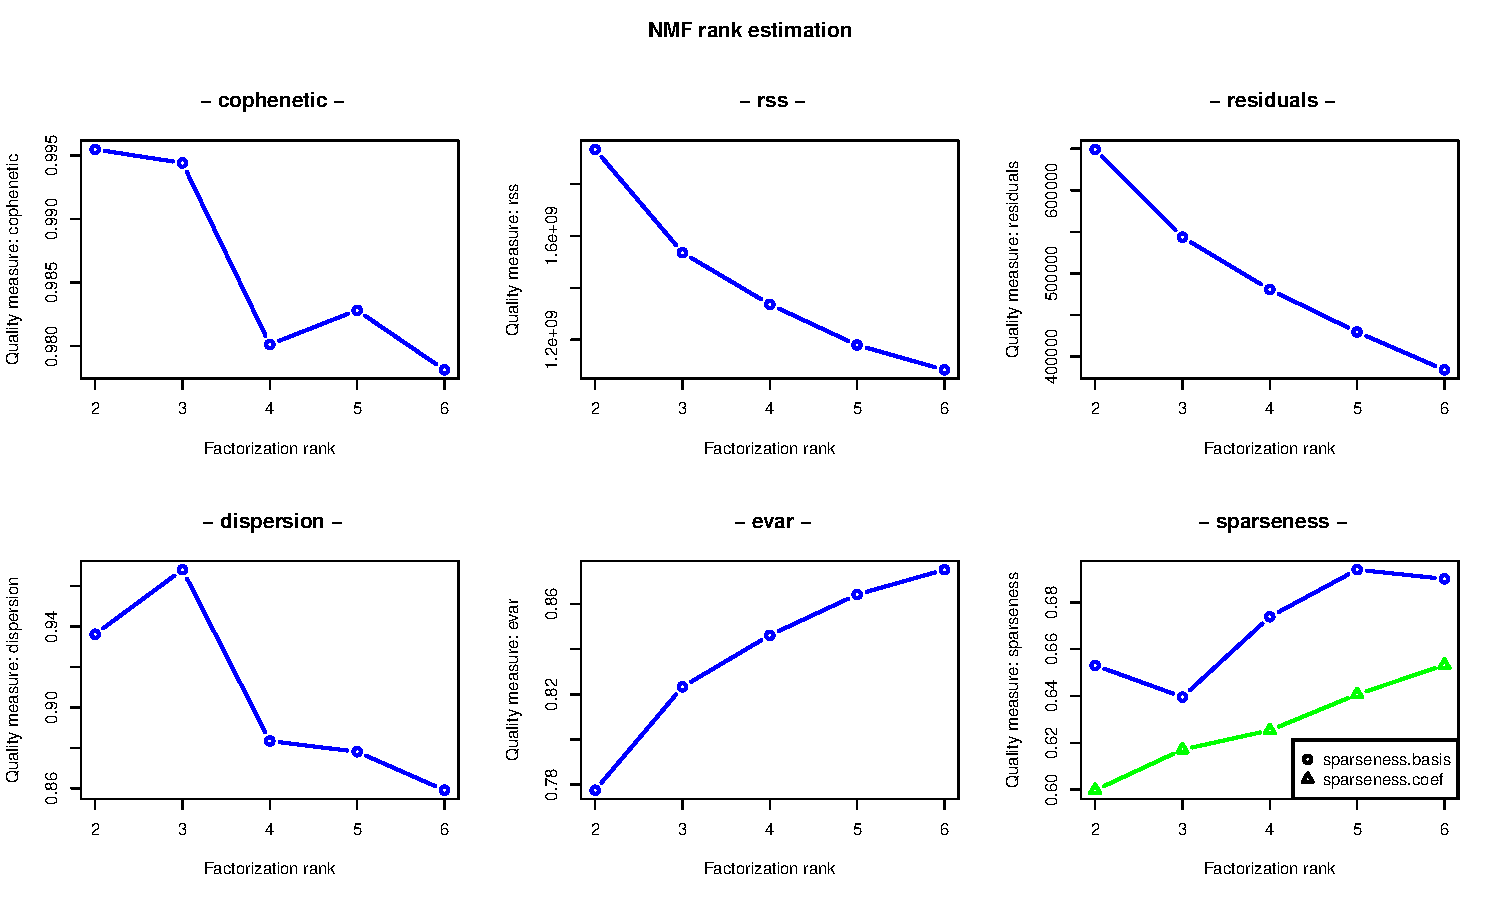
\includegraphics[width=\maxwidth]{/home/renaud/Documents/projects/NMF/pkg/vignettes/figure/NMF-vignette-estimate_rank_plot} 

\end{knitrout}
\caption{Estimation of the rank: Quality measures computed from 10 runs for each value of $r$. \label{fig:estim_all}}
\end{figure}

\begin{figure}
\begin{knitrout}
\definecolor{shadecolor}{rgb}{0.969, 0.969, 0.969}\color{fgcolor}\begin{kframe}
\begin{alltt}
\hlkwd{consensusmap}\hlstd{(estim.r,} \hlkwc{annCol}\hlstd{=esGolub,} \hlkwc{labCol}\hlstd{=}\hlnum{NA}\hlstd{,} \hlkwc{labRow}\hlstd{=}\hlnum{NA}\hlstd{)}
\end{alltt}
\end{kframe}
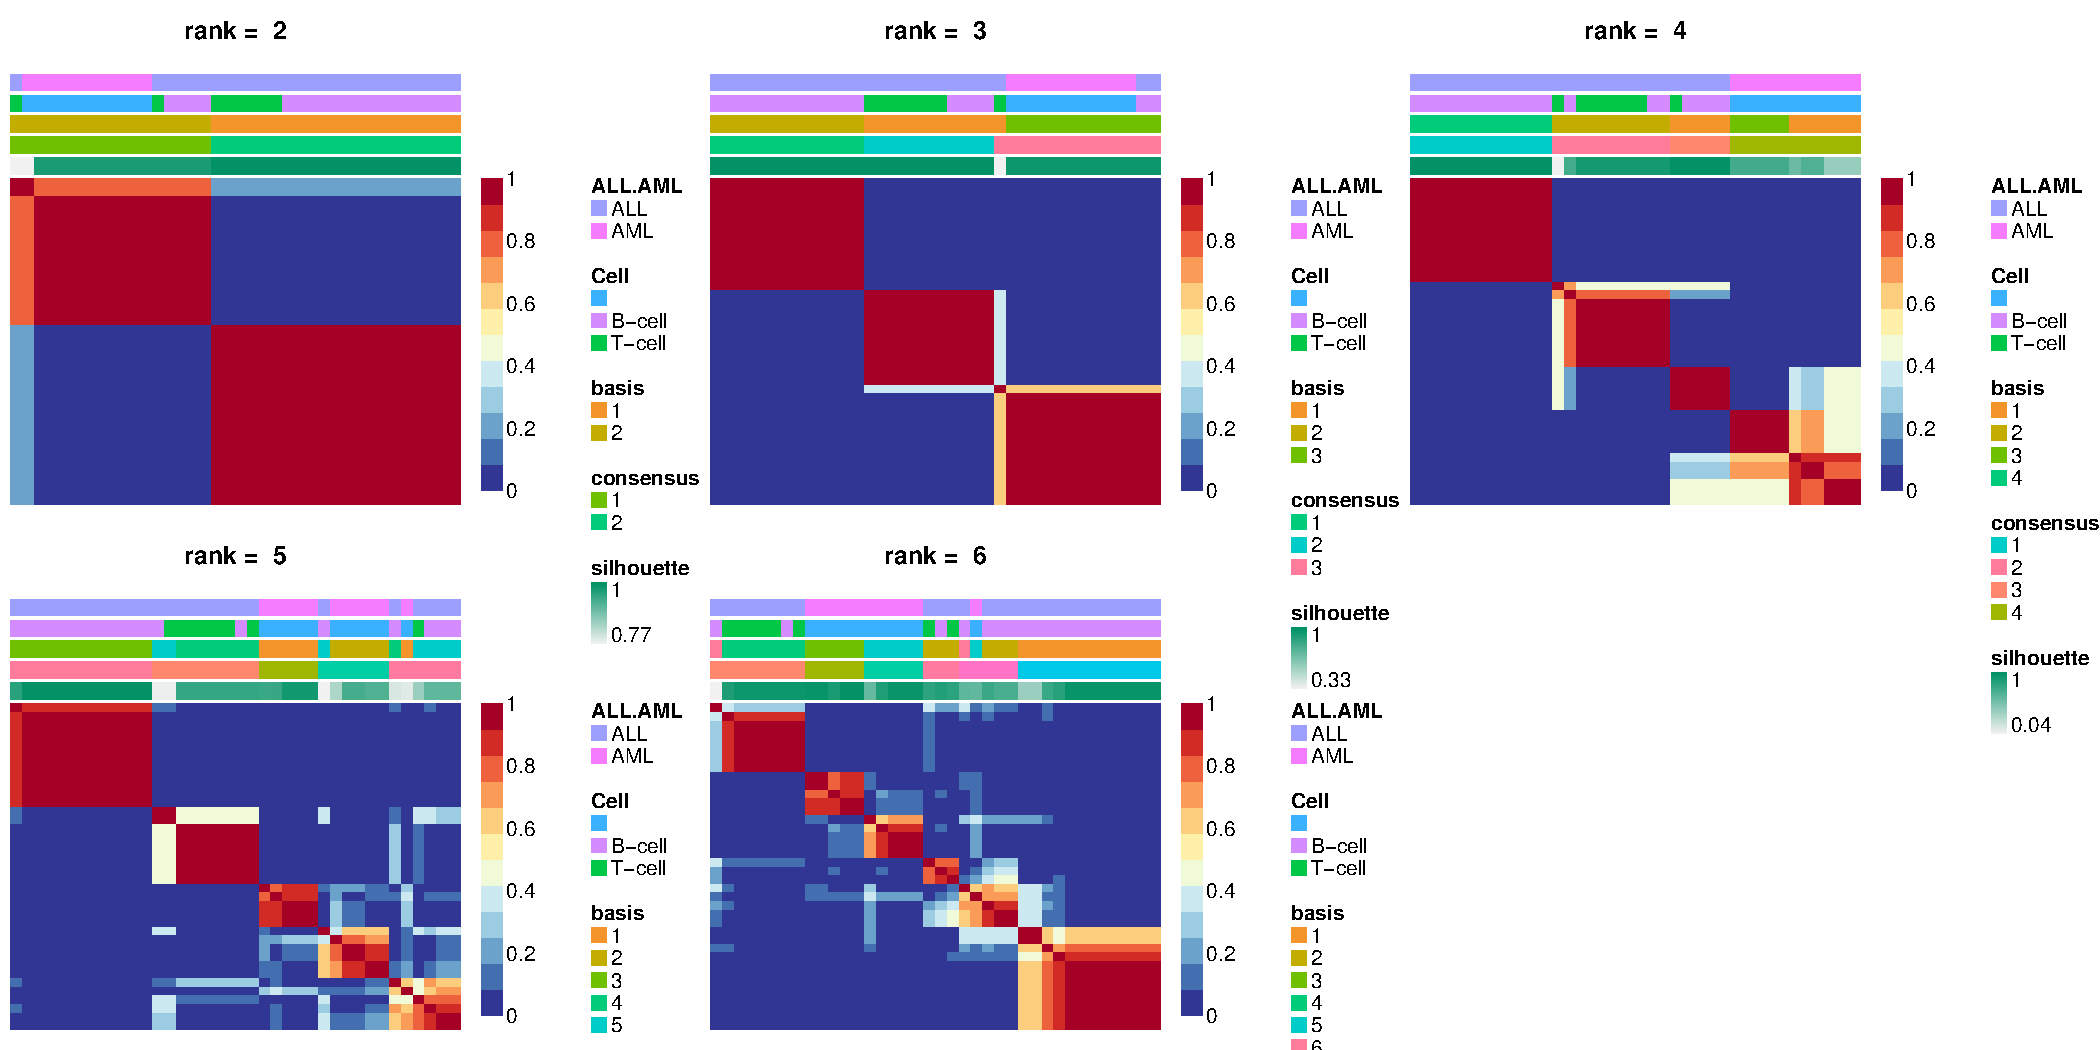
\includegraphics[width=\maxwidth]{/home/renaud/Documents/projects/NMF/pkg/vignettes/figure/NMF-vignette-estimate_rank_hm_include} 

\end{knitrout}
\caption{Estimation of the rank: Consensus matrices computed from 10 runs for each value of $r$. \label{fig:estim_all_hm}}
\end{figure}

\subsubsection{Overfitting}
Even on random data, increasing the factorization rank would lead to decreasing residuals, as more variables are available to better fit the data.
In other words, there is potentially an overfitting problem. 
 
In this context, the approach from \cite{Frigyesi2008} may be useful to prevent or detect overfitting as it takes into account the results for unstructured data.
However it requires to compute the quality measure(s) for the random data.
The \nmfpack package provides a function that shuffles the original data, by permuting the rows of each column, using each time a different permutation.
The rank estimation procedure can then be applied to the randomized data, and the ``random'' measures added to the plot for comparison (\cref{fig:estim_all_rd}).

\begin{figure}
\begin{knitrout}
\definecolor{shadecolor}{rgb}{0.969, 0.969, 0.969}\color{fgcolor}\begin{kframe}
\begin{alltt}
\hlcom{# shuffle original data}
\hlstd{V.random} \hlkwb{<-} \hlkwd{randomize}\hlstd{(esGolub)}
\hlcom{# estimate quality measures from the shuffled data (use default NMF algorithm)}
\hlstd{estim.r.random} \hlkwb{<-} \hlkwd{nmf}\hlstd{(V.random,} \hlnum{2}\hlopt{:}\hlnum{6}\hlstd{,} \hlkwc{nrun}\hlstd{=}\hlnum{10}\hlstd{,} \hlkwc{seed}\hlstd{=}\hlnum{123456}\hlstd{)}
\hlcom{# plot measures on same graph}
\hlkwd{plot}\hlstd{(estim.r, estim.r.random)}
\end{alltt}
\end{kframe}
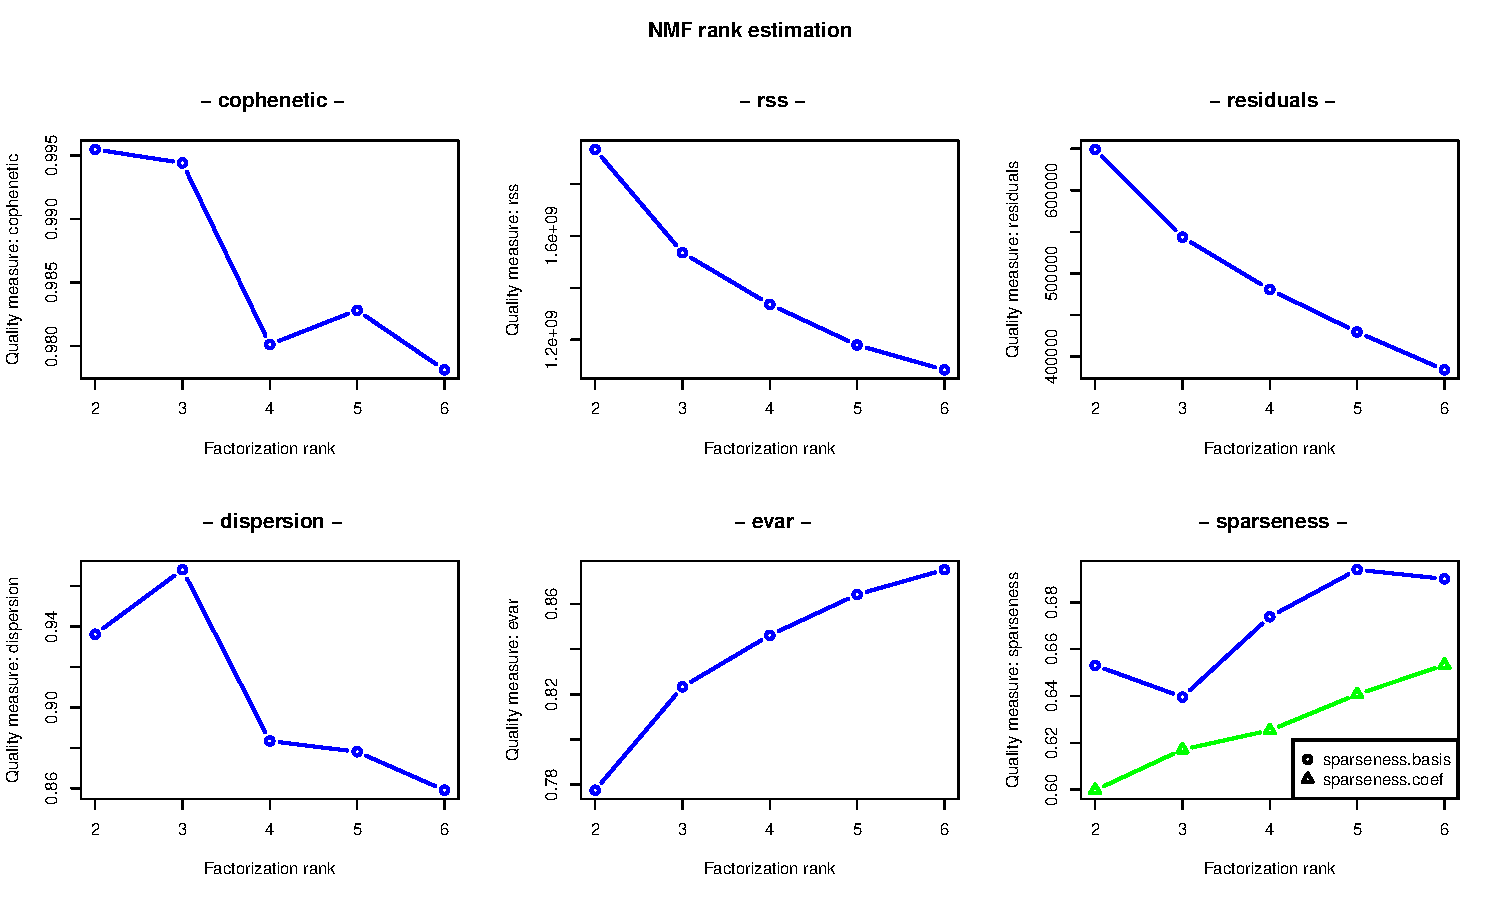
\includegraphics[width=\maxwidth]{/home/renaud/Documents/projects/NMF/pkg/vignettes/figure/NMF-vignette-estimate_rank_random} 

\end{knitrout}
\caption{Estimation of the rank: Comparison of the quality measures with those obtained from randomized data. 
The curves for the actual data are in blue and green, those for the randomized data are in red and pink. 
The estimation is based on Brunet's algorithm.}
\label{fig:estim_all_rd}
\end{figure}

\subsection{Comparing algorithms}
To compare the results from different algorithms, one can pass a list of methods in argument \code{method}. 
To enable a fair comparison, a deterministic seeding method should also be used. 
Here we fix the random seed to 123456. 

\begin{knitrout}
\definecolor{shadecolor}{rgb}{0.969, 0.969, 0.969}\color{fgcolor}\begin{kframe}
\begin{alltt}
\hlcom{# fit a model for several different methods }
\hlstd{res.multi.method} \hlkwb{<-} \hlkwd{nmf}\hlstd{(esGolub,} \hlnum{3}\hlstd{,} \hlkwd{list}\hlstd{(}\hlstr{'brunet'}\hlstd{,} \hlstr{'lee'}\hlstd{,} \hlstr{'ns'}\hlstd{),} \hlkwc{seed}\hlstd{=}\hlnum{123456}\hlstd{,} \hlkwc{.options}\hlstd{=}\hlstr{'t'}\hlstd{)}
\end{alltt}
\begin{verbatim}
## Compute NMF method 'brunet' [1/3] ... OK
## Compute NMF method 'lee' [2/3] ... OK
## Compute NMF method 'ns' [3/3] ... OK
\end{verbatim}
\end{kframe}
\end{knitrout}

Passing the result to method \code{compare} produces a \code{data.frame} that contains summary measures for each method. Again, prior knowledge of classes may be used to compute clustering quality measures:  

\begin{knitrout}
\definecolor{shadecolor}{rgb}{0.969, 0.969, 0.969}\color{fgcolor}\begin{kframe}
\begin{alltt}
\hlkwd{compare}\hlstd{(res.multi.method)}
\end{alltt}
\begin{verbatim}
##        method   seed rng    metric rank sparseness.basis sparseness.coef
## brunet brunet random   1        KL    3           0.6393          0.6218
## lee       lee random   1 euclidean    3           0.7269          0.4466
## nsNMF   nsNMF random   1        KL    3           0.6777          0.7350
##        silhouette.coef silhouette.basis residuals niter   cpu cpu.all nrun
## brunet          0.8126           0.7488    543536   510 0.270   0.270    1
## lee             0.7148           0.6764 673513121  1780 0.982   0.982    1
## nsNMF           0.8654           0.7946    585106   970 0.696   0.696    1
\end{verbatim}
\begin{alltt}
\hlcom{# If prior knowledge of classes is available}
\hlkwd{compare}\hlstd{(res.multi.method,} \hlkwc{class}\hlstd{=esGolub}\hlopt{$}\hlstd{Cell)}
\end{alltt}
\begin{verbatim}
##        method   seed rng    metric rank sparseness.basis sparseness.coef
## brunet brunet random   1        KL    3           0.6393          0.6218
## lee       lee random   1 euclidean    3           0.7269          0.4466
## nsNMF   nsNMF random   1        KL    3           0.6777          0.7350
##        purity entropy silhouette.coef silhouette.basis residuals niter
## brunet 0.8158  0.3927          0.8126           0.7488    543536   510
## lee    0.5789  0.7231          0.7148           0.6764 673513121  1780
## nsNMF  0.7895  0.4691          0.8654           0.7946    585106   970
##          cpu cpu.all nrun
## brunet 0.270   0.270    1
## lee    0.982   0.982    1
## nsNMF  0.696   0.696    1
\end{verbatim}
\end{kframe}
\end{knitrout}

Because the computation was performed with error tracking enabled, an error plot
can be produced by method \code{plot} (\cref{fig:errorplot}).
Each track is normalized so that its first value equals one, and stops at the iteration where the method's convergence criterion was fulfilled.

\subsection{Visualization methods}

\subsubsection*{Error track}

If the NMF computation is performed with error tracking enabled -- using argument \code{.options} -- the trajectory of the objective value is computed during the fit.
This computation is not enabled by default as it induces some overhead. 

\begin{knitrout}
\definecolor{shadecolor}{rgb}{0.969, 0.969, 0.969}\color{fgcolor}\begin{kframe}
\begin{alltt}
\hlcom{# run nmf with .option='t'}
\hlstd{res} \hlkwb{<-} \hlkwd{nmf}\hlstd{(esGolub,} \hlnum{3}\hlstd{,} \hlkwc{.options}\hlstd{=}\hlstr{'t'}\hlstd{)}
\hlcom{# or with .options=list(track=TRUE)}
\end{alltt}
\end{kframe}
\end{knitrout}

The trajectory can be plot with the method \code{plot} (\cref{fig:errorplot}):
\begin{figure}[!htbp]
\begin{knitrout}
\definecolor{shadecolor}{rgb}{0.969, 0.969, 0.969}\color{fgcolor}\begin{kframe}
\begin{alltt}
\hlkwd{plot}\hlstd{(res)}
\hlkwd{plot}\hlstd{(res.multi.method)}
\end{alltt}
\end{kframe}
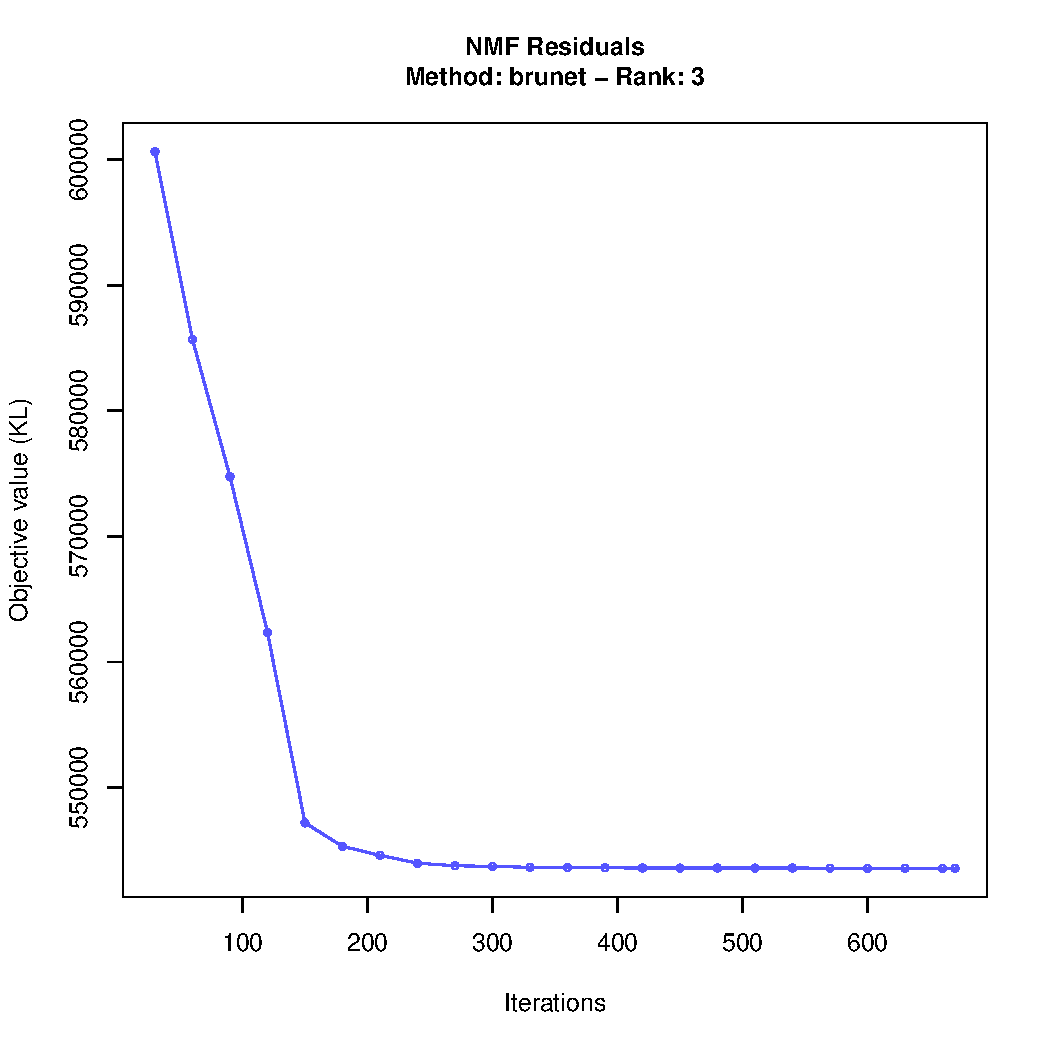
\includegraphics[width=0.5\textwidth]{/home/renaud/Documents/projects/NMF/pkg/vignettes/figure/NMF-vignette-errorplot1} 
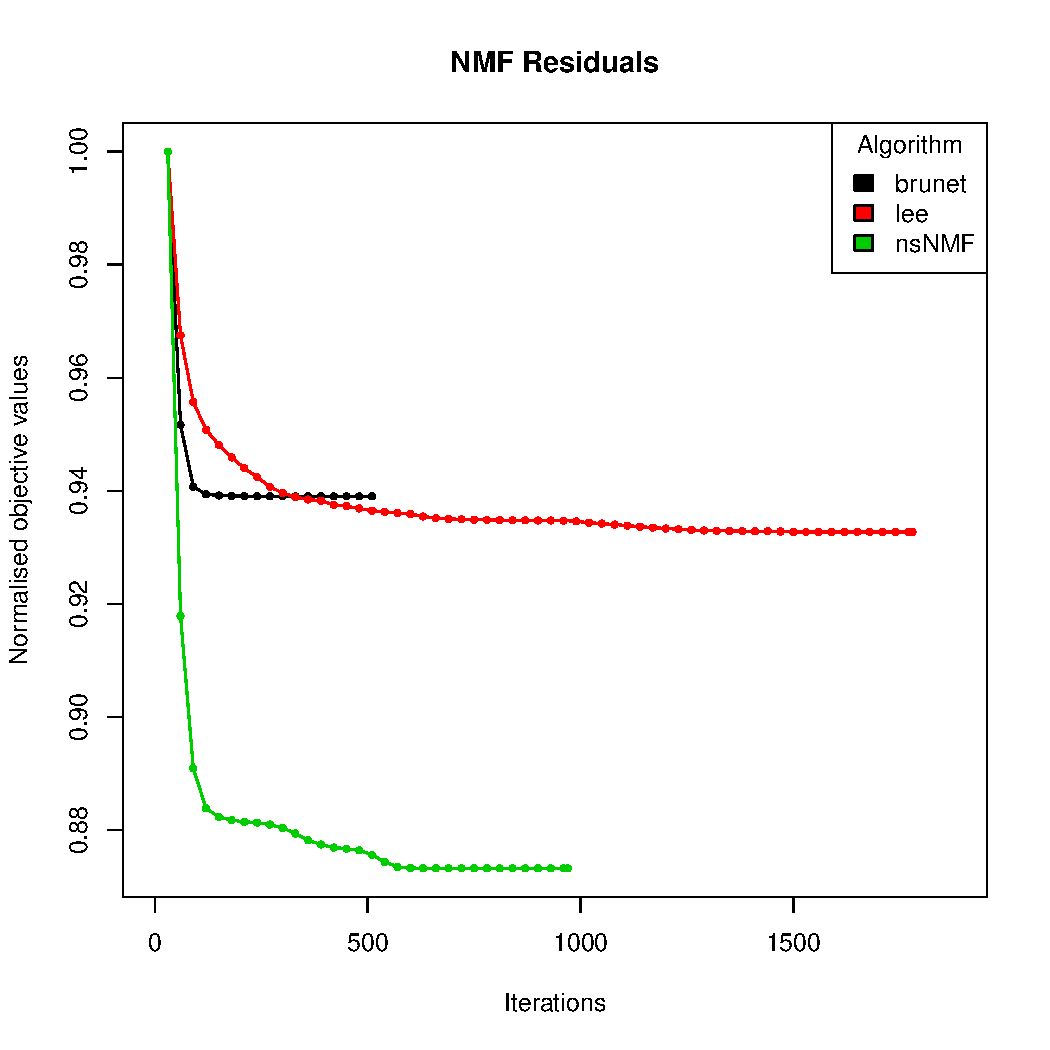
\includegraphics[width=0.5\textwidth]{/home/renaud/Documents/projects/NMF/pkg/vignettes/figure/NMF-vignette-errorplot2} 

\end{knitrout}
\caption{Error track for a single NMF run (left) and multiple method
runs (right)}
\label{fig:errorplot}
\end{figure}

\subsubsection*{Heatmaps}

The methods \code{basismap}, \code{coefmap} and \code{consensusmap} provide an
easy way to visualize respectively the resulting basis matrix (i.e. metagenes),
mixture coefficient matrix (i.e. metaprofiles) and the consensus matrix, in the
case of multiple runs.
It produces pre-configured heatmaps based on the function \code{aheatmap}, the
underlying heatmap engine provided with the package NMF. 
The default heatmaps produced by these functions are shown in
\cref{fig:heatmap_coef_basis,fig:heatmap_consensus}.
They can be customized in many different ways (colours, annotations, labels).
See the dedicated vignette \emph{``NMF: generating heatmaps"} or the help pages
\code{?coefmap} and \code{?aheatmap} for more information.

An important and unique feature of the function \code{aheatmap}, is that it
makes it possible to combine several heatmaps on the same plot, using the both
standard layout calls \texttt{par(mfrow=...)} and \texttt{layout(...)}, or grid
viewports from \texttt{grid} graphics.
The plotting context is automatically internally detected, and a correct
behaviour is achieved thanks to the \citeCRANpkg{gridBase}.
Examples are provided in the dedicated vignette mentioned above.

The rows of the basis matrix often carry the high dimensionality of the data: genes, loci, pixels, features, etc\ldots 
The function \code{basismap} extends the use of argument \code{subsetRow} (from \code{aheatmap}) to the specification of a feature selection method.
In \cref{fig:heatmap_coef_basis} we simply used \code{subsetRow=TRUE}, which subsets the rows using the method described in \cite{KimH2007}, to only keep the basis-specific features (e.g. the metagene-specific genes). 
We refer to the relevant help pages \code{?basismap} and \code{?aheatmap} for more details about other possible values for this argument.

\begin{figure}[!htbp]
\centering
\begin{knitrout}
\definecolor{shadecolor}{rgb}{0.969, 0.969, 0.969}\color{fgcolor}\begin{kframe}
\begin{alltt}
\hlkwd{layout}\hlstd{(}\hlkwd{cbind}\hlstd{(}\hlnum{1}\hlstd{,}\hlnum{2}\hlstd{))}
\hlcom{# basis components}
\hlkwd{basismap}\hlstd{(res,} \hlkwc{subsetRow}\hlstd{=}\hlnum{TRUE}\hlstd{)}
\hlcom{# mixture coefficients}
\hlkwd{coefmap}\hlstd{(res)}
\end{alltt}
\end{kframe}
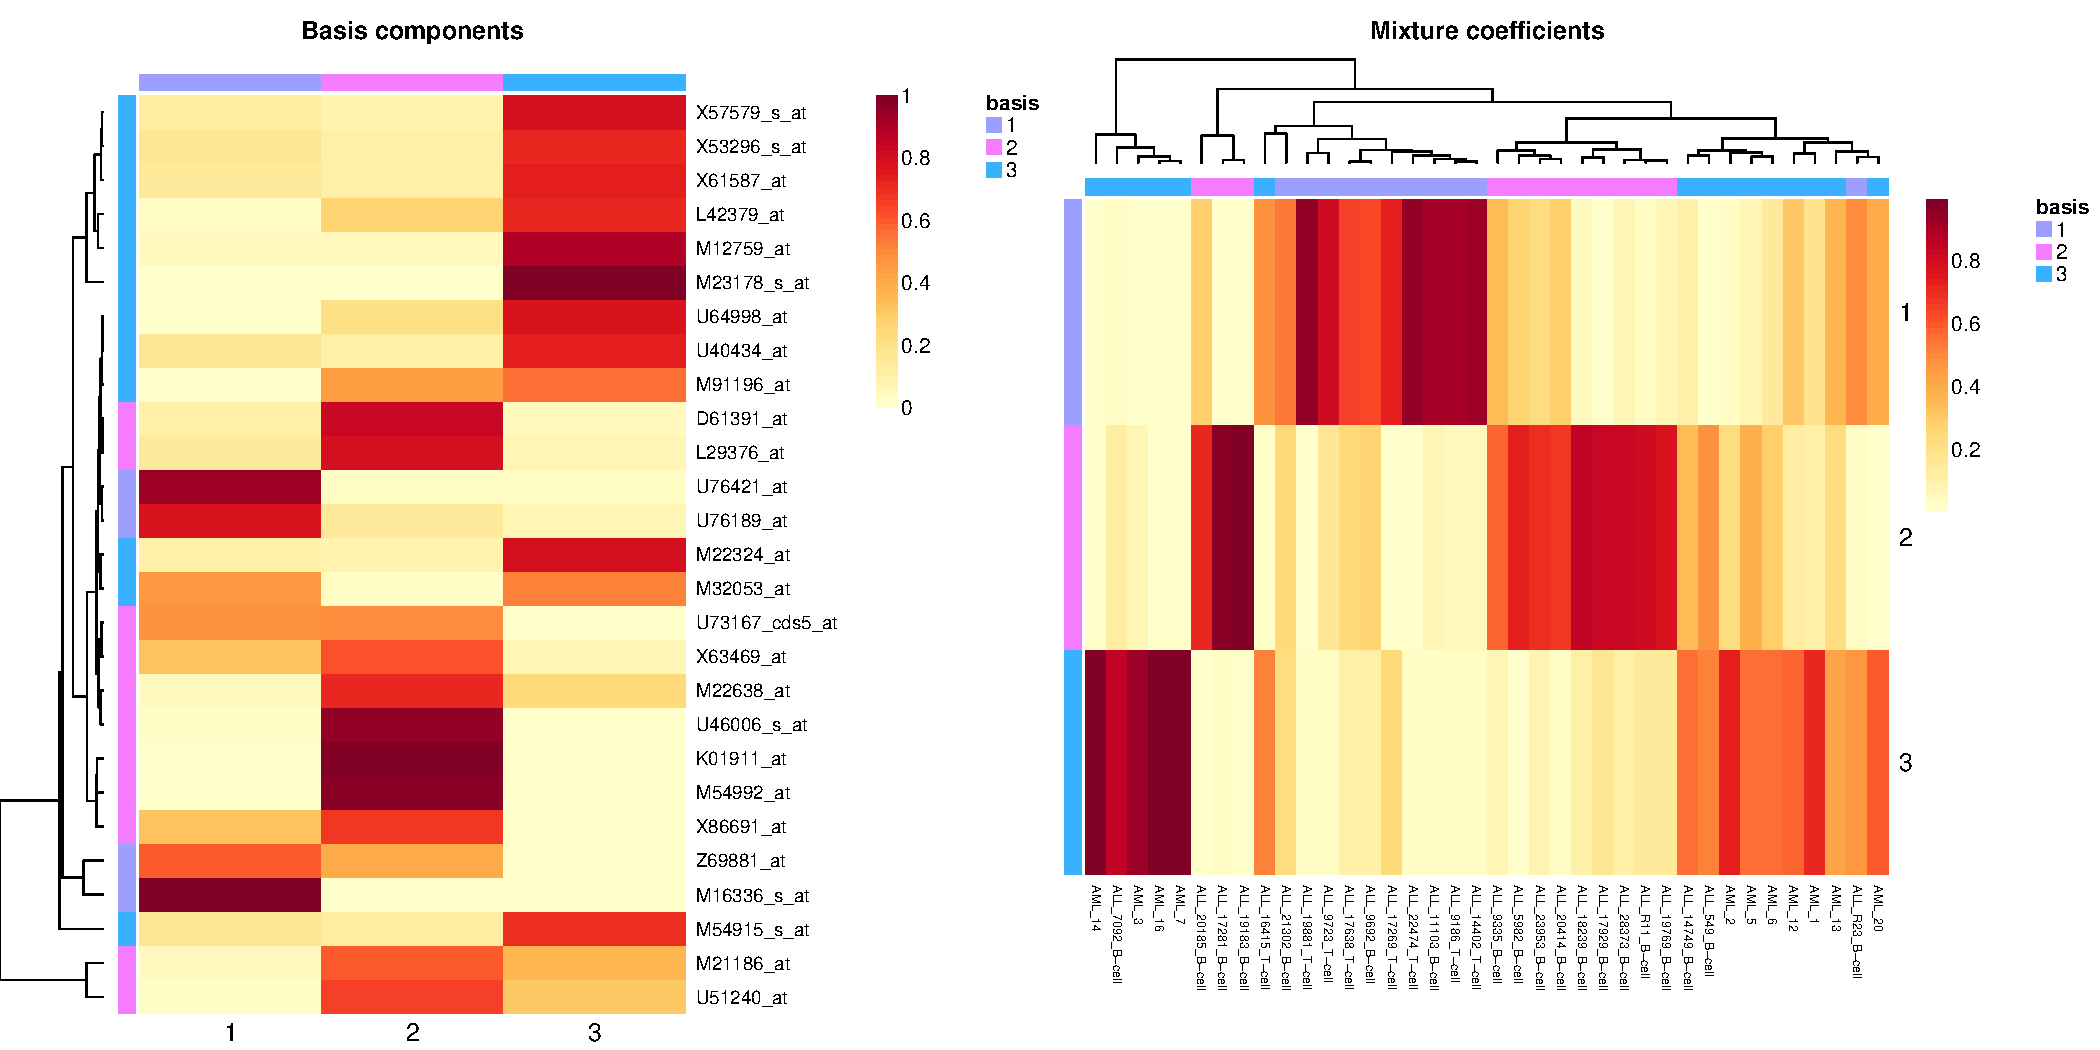
\includegraphics[width=\maxwidth]{/home/renaud/Documents/projects/NMF/pkg/vignettes/figure/NMF-vignette-heatmap_coef_basis_inc} 

\end{knitrout}
\caption{Heatmap of the basis and the mixture coefficient matrices. The rows of the basis matrix were selected using the default feature selection method -- described in \cite{KimH2007}.}
\label{fig:heatmap_coef_basis}
\end{figure}

In the case of multiple runs the function \code{consensusmap} plots the consensus matrix, i.e. the average connectivity matrix across the runs (see results in \cref{fig:heatmap_consensus} for a consensus matrix obtained with 100 runs of Brunet's algorithm on the complete 
Golub dataset):

\begin{figure}[ht]
\begin{knitrout}
\definecolor{shadecolor}{rgb}{0.969, 0.969, 0.969}\color{fgcolor}\begin{kframe}
\begin{alltt}
\hlcom{# The cell type is used to label rows and columns }
\hlkwd{consensusmap}\hlstd{(res.multirun,} \hlkwc{annCol}\hlstd{=esGolub,} \hlkwc{tracks}\hlstd{=}\hlnum{NA}\hlstd{)}
\end{alltt}
\end{kframe}
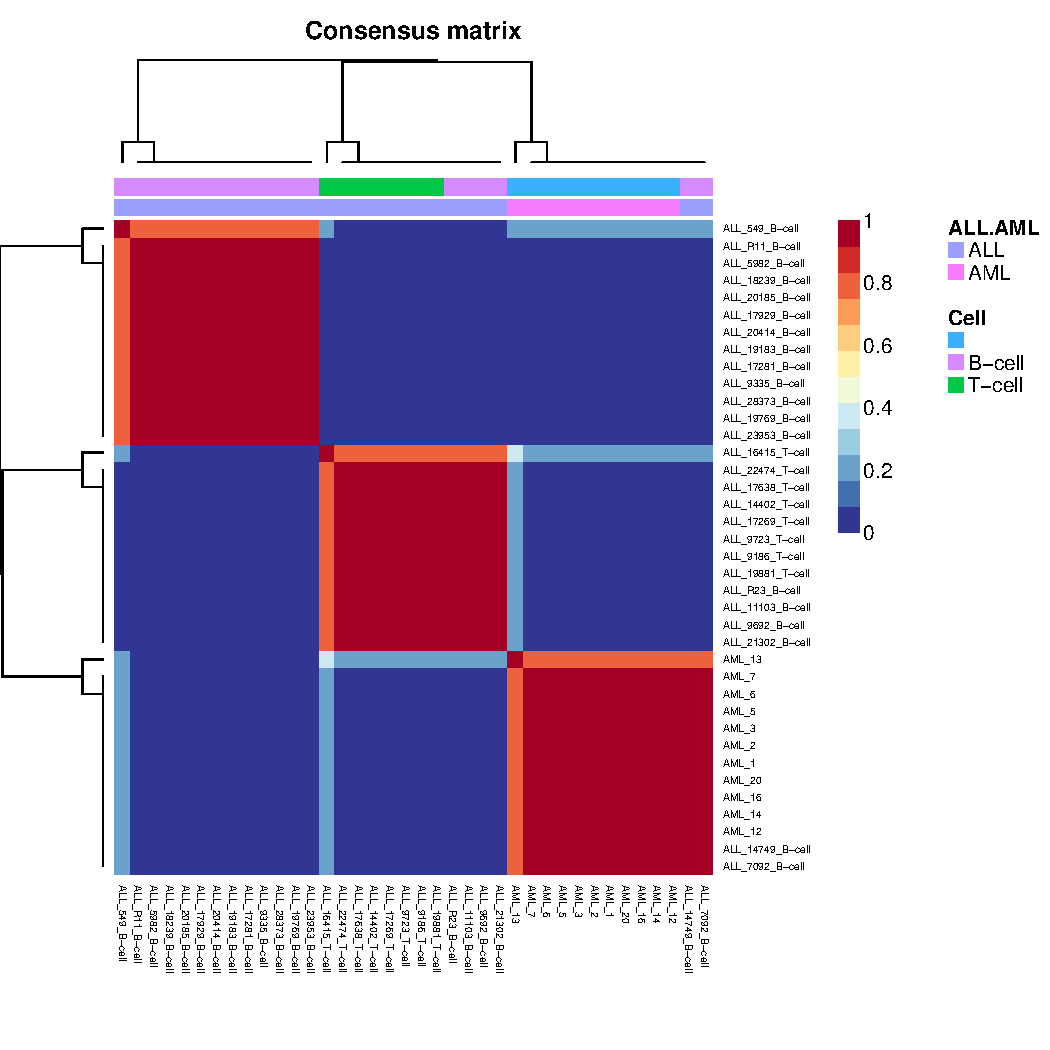
\includegraphics[width=0.49\textwidth]{/home/renaud/Documents/projects/NMF/pkg/vignettes/figure/NMF-vignette-heatmap_consensus_inc1} 

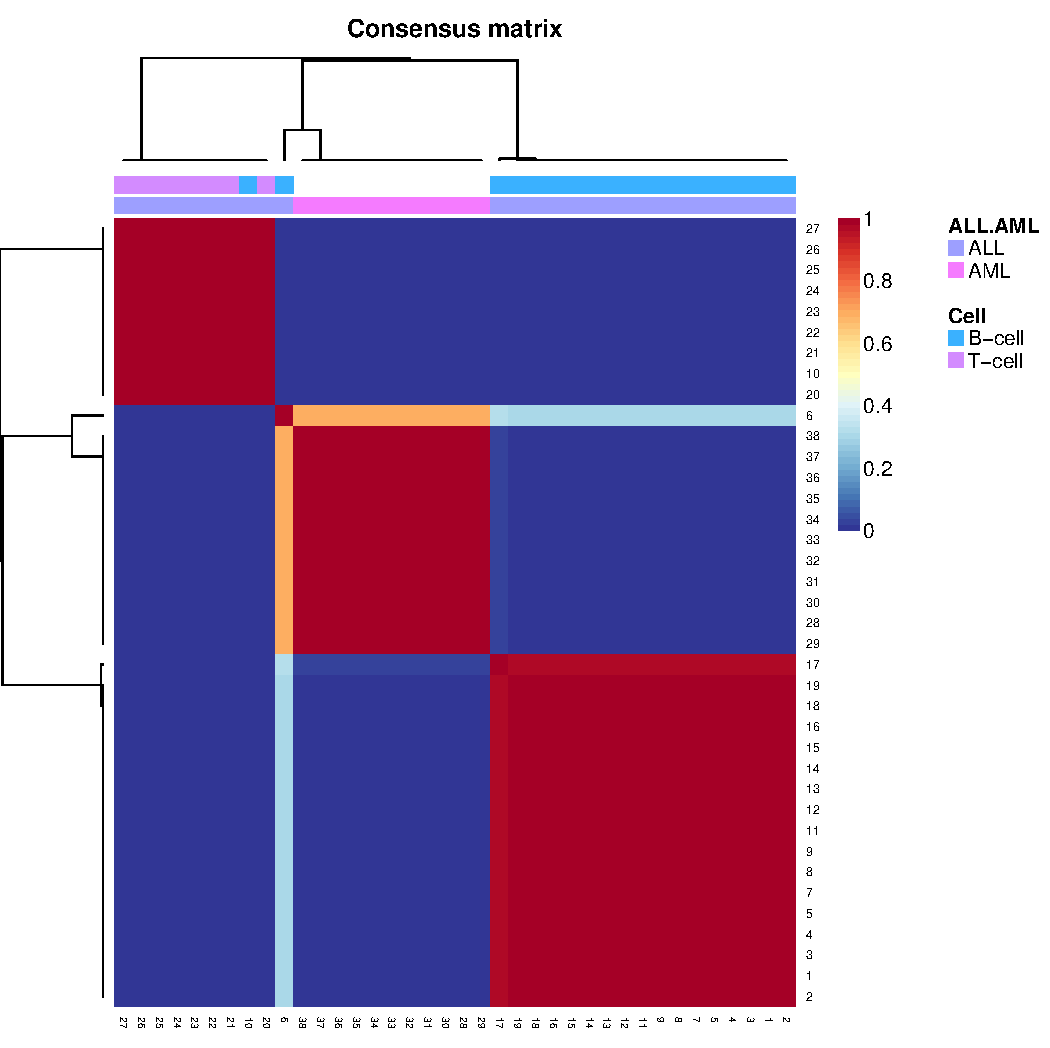
\includegraphics[width=0.49\textwidth]{/home/renaud/Documents/projects/NMF/pkg/vignettes/figure/NMF-vignette-heatmap_consensus_inc2} 

\end{knitrout}

\caption{Heatmap of consensus matrices from 10 runs on the reduced dataset
(left) and from 100 runs on the complete Golub dataset (right).}
\label{fig:heatmap_consensus}
\end{figure}
 
\section{Extending the package}

We developed the \nmfpack\ package with the objective to facilitate the integration of new NMF methods, trying to impose only few requirements on their implementations. 
All the built-in algorithms and seeding methods are implemented as strategies that are called from within the main interface method \code{nmf}. 

The user can define new strategies and those are handled in exactly the same way as the built-in ones, benefiting from the same utility functions to interpret the 
results and assess their performance. 

\subsection{Custom algorithm}
%New NMF algrithms can be defined in two ways:
%
%\begin{itemize}
%\item as a single \code{function} 
%\item as a set of functions that implement a pre-defined \emph{iterative schema}
%\end{itemize}
%
%\subsubsection{Defined as a \code{function}}

\subsubsection{Using a custom algorithm}\label{sec:algo_custom}
To define a strategy, the user needs to provide a \code{function} that implements the complete algotihm. It must be of the form: 

\begin{knitrout}
\definecolor{shadecolor}{rgb}{0.969, 0.969, 0.969}\color{fgcolor}\begin{kframe}
\begin{alltt}
\hlstd{my.algorithm} \hlkwb{<-} \hlkwa{function}\hlstd{(}\hlkwc{x}\hlstd{,} \hlkwc{seed}\hlstd{,} \hlkwc{param.1}\hlstd{,} \hlkwc{param.2}\hlstd{)\{}
        \hlcom{# do something with starting point}
        \hlcom{# ...}

        \hlcom{# return updated starting point}
        \hlkwd{return}\hlstd{(seed)}
\hlstd{\}}
\end{alltt}
\end{kframe}
\end{knitrout}
Where:

\begin{description}
\item[target] is a \code{matrix}; 
\item[start] is an object that inherits from class \code{NMF}. 
This \code{S4} class is used to handle NMF models (matrices \code{W} and \code{H}, objective function, etc\dots);
\item[param.1, param.2] are extra parameters specific to the algorithms;
\end{description}

The function must return an object that inherits from class \code{NMF}.

For example:
\begin{knitrout}
\definecolor{shadecolor}{rgb}{0.969, 0.969, 0.969}\color{fgcolor}\begin{kframe}
\begin{alltt}
\hlstd{my.algorithm} \hlkwb{<-} \hlkwa{function}\hlstd{(}\hlkwc{x}\hlstd{,} \hlkwc{seed}\hlstd{,} \hlkwc{scale.factor}\hlstd{=}\hlnum{1}\hlstd{)\{}
        \hlcom{# do something with starting point}
        \hlcom{# ...}
        \hlcom{# for example: }
        \hlcom{# 1. compute principal components	}
        \hlstd{pca} \hlkwb{<-} \hlkwd{prcomp}\hlstd{(}\hlkwd{t}\hlstd{(x),} \hlkwc{retx}\hlstd{=}\hlnum{TRUE}\hlstd{)}

        \hlcom{# 2. use the absolute values of the first PCs for the metagenes}
        \hlcom{# Note: the factorization rank is stored in object 'start'	}
        \hlstd{factorization.rank} \hlkwb{<-} \hlkwd{nbasis}\hlstd{(seed)}
        \hlkwd{basis}\hlstd{(seed)} \hlkwb{<-} \hlkwd{abs}\hlstd{(pca}\hlopt{$}\hlstd{rotation[,}\hlnum{1}\hlopt{:}\hlstd{factorization.rank])}
        \hlcom{# use the rotated matrix to get the mixture coefficient}
        \hlcom{# use a scaling factor (just to illustrate the use of extra parameters)}
        \hlkwd{coef}\hlstd{(seed)} \hlkwb{<-} \hlkwd{t}\hlstd{(}\hlkwd{abs}\hlstd{(pca}\hlopt{$}\hlstd{x[,}\hlnum{1}\hlopt{:}\hlstd{factorization.rank]))} \hlopt{/} \hlstd{scale.factor}

        \hlcom{# return updated data}
        \hlkwd{return}\hlstd{(seed)}
\hlstd{\}}
\end{alltt}
\end{kframe}
\end{knitrout}

To use the new method within the package framework, one pass \code{my.algorithm} to main interface \code{nmf} via argument \code{method}. 
Here we apply the algorithm to some matrix \code{V} randomly generated: 

\begin{knitrout}
\definecolor{shadecolor}{rgb}{0.969, 0.969, 0.969}\color{fgcolor}\begin{kframe}
\begin{alltt}
\hlstd{n} \hlkwb{<-} \hlnum{50}\hlstd{; r} \hlkwb{<-} \hlnum{3}\hlstd{; p} \hlkwb{<-} \hlnum{20}
\hlstd{V} \hlkwb{<-}\hlkwd{syntheticNMF}\hlstd{(n, r, p)}
\end{alltt}
\end{kframe}
\end{knitrout}

\begin{knitrout}
\definecolor{shadecolor}{rgb}{0.969, 0.969, 0.969}\color{fgcolor}\begin{kframe}
\begin{alltt}
\hlkwd{nmf}\hlstd{(V,} \hlnum{3}\hlstd{, my.algorithm,} \hlkwc{scale.factor}\hlstd{=}\hlnum{10}\hlstd{)}
\end{alltt}
\begin{verbatim}
## <Object of class: NMFfit>
##  # Model:
##   <Object of class:NMFstd>
##   features: 50 
##   basis/rank: 3 
##   samples: 20 
##  # Details:
##   algorithm:  nmf_7ff64043af4a 
##   seed:  random 
##   RNG: 403L, 173L, ..., 1280296329L [0d87fde5bf092083bd059bcc33d58a3e]
##   distance metric:  'euclidean' 
##   residuals:  554.9 
##   parameters: scale.factor=10 
##   Timing:
##      user  system elapsed 
##     0.009   0.000   0.010
\end{verbatim}
\end{kframe}
\end{knitrout}

\subsubsection{Using a custom distance measure}
The default distance measure is based on the euclidean distance. 
If the algorithm is based on another distance measure, this one can be specified in argument \code{objective}, either as a \code{character} string corresponding to a built-in objective function, or a custom \code{function} definition\footnote{Note that from version 0.8, the arguments for custom objective functions have been swapped: (1) the current NMF model, (2) the target matrix}:

\begin{knitrout}
\definecolor{shadecolor}{rgb}{0.969, 0.969, 0.969}\color{fgcolor}\begin{kframe}
\begin{alltt}
\hlcom{# based on Kullback-Leibler divergence}
\hlkwd{nmf}\hlstd{(V,} \hlnum{3}\hlstd{, my.algorithm,} \hlkwc{scale.factor}\hlstd{=}\hlnum{10}\hlstd{,} \hlkwc{objective}\hlstd{=}\hlstr{'KL'}\hlstd{)}
\end{alltt}
\begin{verbatim}
## <Object of class: NMFfit>
##  # Model:
##   <Object of class:NMFstd>
##   features: 50 
##   basis/rank: 3 
##   samples: 20 
##  # Details:
##   algorithm:  nmf_7ff6633562c1 
##   seed:  random 
##   RNG: 403L, 383L, ..., 1280296329L [2f2572f5c6b643d37859d97079951964]
##   distance metric:  'KL' 
##   residuals:  1539 
##   parameters: scale.factor=10 
##   Timing:
##      user  system elapsed 
##     0.005   0.000   0.006
\end{verbatim}
\begin{alltt}
\hlcom{# based on custom distance metric}
\hlkwd{nmf}\hlstd{(V,} \hlnum{3}\hlstd{, my.algorithm,} \hlkwc{scale.factor}\hlstd{=}\hlnum{10}
        \hlstd{,} \hlkwc{objective}\hlstd{=}\hlkwa{function}\hlstd{(}\hlkwc{model}\hlstd{,} \hlkwc{target}\hlstd{,} \hlkwc{...}\hlstd{)\{}
            \hlstd{(} \hlkwd{sum}\hlstd{( (target}\hlopt{-}\hlkwd{fitted}\hlstd{(model))}\hlopt{^}\hlnum{4} \hlstd{) )}\hlopt{^}\hlstd{\{}\hlnum{1}\hlopt{/}\hlnum{4}\hlstd{\}}
                \hlstd{\}}
\hlstd{)}
\end{alltt}
\begin{verbatim}
## <Object of class: NMFfit>
##  # Model:
##   <Object of class:NMFstd>
##   features: 50 
##   basis/rank: 3 
##   samples: 20 
##  # Details:
##   algorithm:  nmf_7ff62fae0207 
##   seed:  random 
##   RNG: 403L, 593L, ..., 1280296329L [7ed64fa772a4b1e68cebc0bfed3cb018]
##   distance metric:  <function> 
##   residuals:  9.181 
##   parameters: scale.factor=10 
##   Timing:
##      user  system elapsed 
##     0.006   0.000   0.005
\end{verbatim}
\end{kframe}
\end{knitrout}

%\subsubsection{Using the iterative schema} 
%
%NMF algorithms generally implement the following common iterative schema:
%
%\begin{enumerate}
%\item
%\item 
%\end{enumerate}

\subsubsection{Defining algorithms for mixed sign data}
All the algorithms implemented in the \nmfpack package assume that the input data is nonnegative.
However, some methods exist in the litterature that work with relaxed constraints, where the input data and one of the matrix factors ($W$ or $H$) are allowed to have negative entries (eg. semi-NMF \cite{Ding2010, Roux2008}).
Strictly speaking these methods do not fall into the NMF category, but still solve constrained matrix factorization problems, and could be considered as NMF methods when applied to non-negative data.
Moreover, we received user requests to enable the development of semi-NMF type methods within the package's framework.
Therefore, we designed the \nmfpack package so that such algorithms -- that handle negative data -- can be integrated. This section documents how to do it.

By default, as a safe-guard, the sign of the input data is checked before running any method, so that the \code{nmf} function throws an error if applied to data that contain negative entries \footnote{Note that on the other side, the sign of the factors returned by the algorithms is never checked, so that one can always return factors with negative entries.}.
To extend the capabilities of the \nmfpack package in handling negative data, and plug mixed sign NMF methods into the framework, the user needs to specify the argument \code{mixed=TRUE} in the call to the \code{nmf} function.
This will skip the sign check of the input data and let the custom algorithm perform the factorization.
 
As an example, we reuse the previously defined custom algorithm\footnote{As it is defined here, the custom algorithm still returns nonnegative factors, which would not be desirable in a real example, as one would not be able to closely fit the negative entries.}:

\begin{knitrout}
\definecolor{shadecolor}{rgb}{0.969, 0.969, 0.969}\color{fgcolor}\begin{kframe}
\begin{alltt}
\hlcom{# put some negative input data }
\hlstd{V.neg} \hlkwb{<-} \hlstd{V; V.neg[}\hlnum{1}\hlstd{,]} \hlkwb{<-} \hlopt{-}\hlnum{1}\hlstd{;}

\hlcom{# this generates an error}
\hlkwd{try}\hlstd{(} \hlkwd{nmf}\hlstd{(V.neg,} \hlnum{3}\hlstd{, my.algorithm,} \hlkwc{scale.factor}\hlstd{=}\hlnum{10}\hlstd{) )}
\end{alltt}


{\ttfamily\noindent\bfseries\color{errorcolor}{\#\# Error: NMF::nmf - Input matrix x contains some negative entries.}}\begin{alltt}
\hlcom{# this runs my.algorithm without error}
\hlkwd{nmf}\hlstd{(V.neg,} \hlnum{3}\hlstd{, my.algorithm,} \hlkwc{mixed}\hlstd{=}\hlnum{TRUE}\hlstd{,} \hlkwc{scale.factor}\hlstd{=}\hlnum{10}\hlstd{)}
\end{alltt}
\begin{verbatim}
## <Object of class: NMFfit>
##  # Model:
##   <Object of class:NMFstd>
##   features: 50 
##   basis/rank: 3 
##   samples: 20 
##  # Details:
##   algorithm:  nmf_7ff65431a6e2 
##   seed:  random 
##   RNG: 403L, 179L, ..., -818492466L [850b670d66e22c6d00f5d79570d1ce8a]
##   distance metric:  'euclidean' 
##   residuals:  561.4 
##   parameters: scale.factor=10 
##   Timing:
##      user  system elapsed 
##     0.007   0.000   0.007
\end{verbatim}
\end{kframe}
\end{knitrout}

\subsubsection{Specifying the NMF model}
If not specified in the call, the NMF model that is used is the standard one, as defined in \cref{NMFstd}. 
However, some NMF algorithms have different underlying models, such as non-smooth NMF \cite{Pascual-Montano2006} which uses an extra matrix factor that introduces an extra parameter, and change the way the target matrix is approximated.

The NMF models are defined as S4 classes that extends class \code{NMF}. All the available models can be retreived calling the \code{nmfModel()} function with no 
argument:

\begin{knitrout}
\definecolor{shadecolor}{rgb}{0.969, 0.969, 0.969}\color{fgcolor}\begin{kframe}
\begin{alltt}
\hlkwd{nmfModel}\hlstd{()}
\end{alltt}
\begin{verbatim}
## <Object of class:NMFstd>
## features: 0 
## basis/rank: 0 
## samples: 0
\end{verbatim}
\end{kframe}
\end{knitrout}
 
One can specify the NMF model to use with a custom algorithm, using argument \code{model}. Here we first adapt a bit the custom algorithm, to justify and illustrate the use of a different model.
We use model \code{NMFOffset} \cite{Badea2008}, that includes an offset to take into account genes that have constant expression levels accross the samples:

\begin{knitrout}
\definecolor{shadecolor}{rgb}{0.969, 0.969, 0.969}\color{fgcolor}\begin{kframe}
\begin{alltt}
\hlstd{my.algorithm.offset} \hlkwb{<-} \hlkwa{function}\hlstd{(}\hlkwc{x}\hlstd{,} \hlkwc{seed}\hlstd{,} \hlkwc{scale.factor}\hlstd{=}\hlnum{1}\hlstd{)\{}
        \hlcom{# do something with starting point}
        \hlcom{# ...}
        \hlcom{# for example: }
        \hlcom{# 1. compute principal components	}
        \hlstd{pca} \hlkwb{<-} \hlkwd{prcomp}\hlstd{(}\hlkwd{t}\hlstd{(x),} \hlkwc{retx}\hlstd{=}\hlnum{TRUE}\hlstd{)}

        \hlcom{# retrieve the model being estimated}
        \hlstd{data.model} \hlkwb{<-} \hlkwd{fit}\hlstd{(seed)}

        \hlcom{# 2. use the absolute values of the first PCs for the metagenes}
        \hlcom{# Note: the factorization rank is stored in object 'start'	}
        \hlstd{factorization.rank} \hlkwb{<-} \hlkwd{nbasis}\hlstd{(data.model)}
        \hlkwd{basis}\hlstd{(data.model)} \hlkwb{<-} \hlkwd{abs}\hlstd{(pca}\hlopt{$}\hlstd{rotation[,}\hlnum{1}\hlopt{:}\hlstd{factorization.rank])}
        \hlcom{# use the rotated matrix to get the mixture coefficient}
        \hlcom{# use a scaling factor (just to illustrate the use of extra parameters)}
        \hlkwd{coef}\hlstd{(data.model)} \hlkwb{<-} \hlkwd{t}\hlstd{(}\hlkwd{abs}\hlstd{(pca}\hlopt{$}\hlstd{x[,}\hlnum{1}\hlopt{:}\hlstd{factorization.rank]))} \hlopt{/} \hlstd{scale.factor}

        \hlcom{# 3. Compute the offset as the mean expression}
        \hlstd{data.model}\hlopt{@}\hlkwc{offset} \hlkwb{<-} \hlkwd{rowMeans}\hlstd{(x)}

        \hlcom{# return updated data}
        \hlkwd{fit}\hlstd{(seed)} \hlkwb{<-} \hlstd{data.model}
        \hlstd{seed}
\hlstd{\}}
\end{alltt}
\end{kframe}
\end{knitrout}

Then run the algorithm specifying it needs model \code{NMFOffset}:
\begin{knitrout}
\definecolor{shadecolor}{rgb}{0.969, 0.969, 0.969}\color{fgcolor}\begin{kframe}
\begin{alltt}
\hlcom{# run custom algorithm with NMF model with offset}
\hlkwd{nmf}\hlstd{(V,} \hlnum{3}\hlstd{, my.algorithm.offset,} \hlkwc{model}\hlstd{=}\hlstr{'NMFOffset'}\hlstd{,} \hlkwc{scale.factor}\hlstd{=}\hlnum{10}\hlstd{)}
\end{alltt}
\begin{verbatim}
## <Object of class: NMFfit>
##  # Model:
##   <Object of class:NMFOffset>
##   features: 50 
##   basis/rank: 3 
##   samples: 20 
##   offset: [ 0.3677 0.9383 1.347 1.019 0.6695 ... ]
##  # Details:
##   algorithm:  nmf_7ff6455ba364 
##   seed:  random 
##   RNG: 403L, 389L, ..., -818492466L [7d13c1cc60f9b6390bf7ebfc74dce591]
##   distance metric:  'euclidean' 
##   residuals:  334.3 
##   parameters: scale.factor=10 
##   Timing:
##      user  system elapsed 
##     0.005   0.000   0.005
\end{verbatim}
\end{kframe}
\end{knitrout}


\subsection{Custom seeding method}\label{sec:seed_custom}

The user can also define custom seeding method as a function of the form:


\begin{knitrout}
\definecolor{shadecolor}{rgb}{0.969, 0.969, 0.969}\color{fgcolor}\begin{kframe}
\begin{alltt}
\hlcom{# start: object of class NMF}
\hlcom{# target: the target matrix}
\hlstd{my.seeding.method} \hlkwb{<-} \hlkwa{function}\hlstd{(}\hlkwc{model}\hlstd{,} \hlkwc{target}\hlstd{)\{}

        \hlcom{# use only the largest columns for W}
        \hlstd{w.cols} \hlkwb{<-} \hlkwd{apply}\hlstd{(target,} \hlnum{2}\hlstd{,} \hlkwa{function}\hlstd{(}\hlkwc{x}\hlstd{)} \hlkwd{sqrt}\hlstd{(}\hlkwd{sum}\hlstd{(x}\hlopt{^}\hlnum{2}\hlstd{)))}
        \hlkwd{basis}\hlstd{(model)} \hlkwb{<-} \hlstd{target[,}\hlkwd{order}\hlstd{(w.cols)[}\hlnum{1}\hlopt{:}\hlkwd{nbasis}\hlstd{(model)]]}

        \hlcom{# initialize H randomly}
        \hlkwd{coef}\hlstd{(model)} \hlkwb{<-} \hlkwd{matrix}\hlstd{(}\hlkwd{runif}\hlstd{(}\hlkwd{nbasis}\hlstd{(model)}\hlopt{*}\hlkwd{ncol}\hlstd{(target))}
                                                \hlstd{,} \hlkwd{nbasis}\hlstd{(model),} \hlkwd{ncol}\hlstd{(target))}

        \hlcom{# return updated object}
        \hlkwd{return}\hlstd{(model)}
\hlstd{\}}
\end{alltt}
\end{kframe}
\end{knitrout}

To use the new seeding method:
\begin{knitrout}
\definecolor{shadecolor}{rgb}{0.969, 0.969, 0.969}\color{fgcolor}\begin{kframe}
\begin{alltt}
\hlkwd{nmf}\hlstd{(V,} \hlnum{3}\hlstd{,} \hlstr{'snmf/r'}\hlstd{,} \hlkwc{seed}\hlstd{=my.seeding.method)}
\end{alltt}
\begin{verbatim}
## <Object of class: NMFfit>
##  # Model:
##   <Object of class:NMFstd>
##   features: 50 
##   basis/rank: 3 
##   samples: 20 
##  # Details:
##   algorithm:  snmf/r 
##   seed:  NMF.seed.7ff610d5f053 
##   RNG: 403L, 25L, ..., -1308220775L [e0cc5847b800083c2460eb9eaa25bd4e]
##   distance metric:  <function> 
##   residuals:  195.6 
##   Iterations: 105 
##   Timing:
##      user  system elapsed 
##     0.264   0.003   0.267
\end{verbatim}
\end{kframe}
\end{knitrout}

\section{Advanced usage}

\subsection{Package specific options}
The package specific options can be retieved or changed using the \code{nmf.getOption} and \code{nmf.options} functions. 
These behave similarly as the \code{getOption} and \code{nmf.options} base functions:

\begin{knitrout}
\definecolor{shadecolor}{rgb}{0.969, 0.969, 0.969}\color{fgcolor}\begin{kframe}
\begin{alltt}
\hlcom{#show default algorithm and seeding method}
\hlkwd{nmf.options}\hlstd{(}\hlstr{'default.algorithm'}\hlstd{,} \hlstr{'default.seed'}\hlstd{)}
\end{alltt}
\begin{verbatim}
## $default.algorithm
## [1] "brunet"
## 
## $default.seed
## [1] "random"
\end{verbatim}
\begin{alltt}
\hlcom{# retrieve a single option}
\hlkwd{nmf.getOption}\hlstd{(}\hlstr{'default.seed'}\hlstd{)}
\end{alltt}
\begin{verbatim}
## [1] "random"
\end{verbatim}
\begin{alltt}
\hlcom{## # All options}
\hlcom{## nmf.options()}
\end{alltt}
\end{kframe}
\end{knitrout}

Currently the following options are available:


\begin{description}


\item[cores] Default number of cores to use to perform parallel NMF computations.
Note that this option is effectively used only if the global option \code{'cores'} is
not set.
Moreover, the number of cores can also be set at runtime, in the call to \code{nmf},
via arguments \code{.pbackend} or \code{.options} (see \code{nmf} for more details).

\item[default.algorithm] Default NMF algorithm used by the \code{nmf} function when argument
\code{method} is missing.
The value should the key of one of the registered NMF algorithms or a valid specification of an NMF algorithm.
See \code{?nmfAlgorithm}.

\item[default.seed] Default seeding method used by the \code{nmf} function when argument \code{seed} is missing.
The value should the key of one of the registered seeding methods or a vallid specification of a seeding method.
See \code{?nmfSeed}.

\item[track] Toggle default residual tracking.
When \code{TRUE}, the \code{nmf} function compute and store the residual track in the result -- if not otherwise specified in argument \code{.options}.
Note that tracking may significantly slow down the computations.

\item[track.interval] Number of iterations between two points in the residual track.
This option is relevant only when residual tracking is enabled.
See \code{?nmf}.

\item[error.track] this is a symbolic link to option \code{track} for backward compatibility.

\item[pbackend] Default loop/parallel foreach backend used by the \code{nmf} function when
argument \code{.pbackend} is missing.
Currently the following values are supported: \code{'par'} for multicore,
\code{'seq'} for sequential, \code{NA} for standard \code{sapply} (i.e. do not use a foreach loop),
\code{NULL} for using the currently registered foreach backend.

\item[parallel.backend] this is a symbolic link to option \code{pbackend} for backward compatibility.

\item[gc] Interval/frequency (in number of runs) at which garbage collection is performed.

\item[verbose] Default level of verbosity.

\item[debug] Toogles debug mode.
In this mode the console output may be very -- very -- messy, and is aimed at debugging only.

\item[maxIter]  Default maximum number of iteration to use (default NULL).
This option is for internal/technical usage only, to globally speed up examples or tests
of NMF algorithms. To be used with care at one's own risk...
It is documented here so that advanced users are aware of its existence, and can avoid possible
conflict with their own custom options.


\end{description}
 

The default/current values of each options can be displayed using the function
\code{nmf.printOptions}:

\begin{knitrout}
\definecolor{shadecolor}{rgb}{0.969, 0.969, 0.969}\color{fgcolor}\begin{kframe}
\begin{alltt}
\hlkwd{nmf.printOptions}\hlstd{()}
\end{alltt}
\begin{verbatim}
## <Package specific options: package:NMF>
## Registered: FALSE
## Options:
## List of 13
##  $ default.algorithm: chr "brunet"
##  $ default.seed     : chr "random"
##  $ error.track      :Class 'option_symlink'  chr "track"
##  $ track            : logi FALSE
##  $ track.interval   : num 30
##  $ gc               : num 50
##  $ parallel.backend :Class 'option_symlink'  chr "pbackend"
##  $ pbackend         : chr "par"
##  $ verbose          : logi FALSE
##  $ debug            : logi FALSE
##  $ grid.patch       : logi FALSE
##  $ shared.memory    : logi TRUE
##  $ cores            : num 2
## Defaults:
## List of 12
##  $ default.algorithm: chr "brunet"
##  $ default.seed     : chr "random"
##  $ error.track      :Class 'option_symlink'  chr "track"
##  $ track            : logi FALSE
##  $ track.interval   : num 30
##  $ gc               : num 50
##  $ parallel.backend :Class 'option_symlink'  chr "pbackend"
##  $ pbackend         : chr "par"
##  $ verbose          : logi FALSE
##  $ debug            : logi FALSE
##  $ grid.patch       : logi FALSE
##  $ shared.memory    : logi TRUE
\end{verbatim}
\end{kframe}
\end{knitrout}

%% latex table generated in R 2.10.1 by xtable 1.5-6 package
%% Wed Apr  7 15:27:05 2010
%\begin{table}[ht]
%\begin{center}
%\begin{tabularx}{\textwidth}{>{\ttfamily}rlX}
%  \hline
%Option & Default value & Description\\ 
%\hline
%default.algorithm & brunet & Default NMF algorithm used by the \code{nmf} function when argument \code{method} is missing.
%The value should the key of one of the available NMF algorithms. 
%See \code{?nmfAlgorithm}.\\ 
%track.interval & 30 & Number of iterations between two points in the residual track. 
%This option is relevant only when residual tracking is enabled. 
%See \code{?nmf}.\\ 
%error.track & FALSE & Toggle default residual tracking. 
%When \code{TRUE}, the \code{nmf} function compute and store the residual track in the result -- if not otherwise specified in argument \code{.options}.
%Note that tracking may significantly slow down the computations.\\ 
%default.seed & random & Default seeding method used by the \code{nmf} function when argument \code{seed} is missing.
%The value should the key of one of the available seeding methods. 
%See \code{?nmfSeed}.\\
%backend & mc & Default parallel backend used used by the \code{nmf} function when argument \code{.pbackend} is missing.
%Currently the following values are supported: \code{'mc'} for multicore, \code{'seq'} for sequential, \code{''} for \code{sapply}.\\
%verbose & FALSE & Toggle verbosity.\\ 
%debug & FALSE & Toggle debug mode, which is an extended verbose mode.\\ 
%\hline
%\end{tabularx}
%\end{center}
%\caption{}
%\end{table}

\pagebreak 
\section{Session Info}
\begin{itemize}\raggedright
  \item R version 3.1.1 (2014-07-10), \verb|x86_64-pc-linux-gnu|
  \item Locale: \verb|LC_CTYPE=en_US.UTF-8|, \verb|LC_NUMERIC=C|, \verb|LC_TIME=en_ZA.UTF-8|, \verb|LC_COLLATE=en_US.UTF-8|, \verb|LC_MONETARY=en_ZA.UTF-8|, \verb|LC_MESSAGES=en_US.UTF-8|, \verb|LC_PAPER=en_ZA.UTF-8|, \verb|LC_NAME=C|, \verb|LC_ADDRESS=C|, \verb|LC_TELEPHONE=C|, \verb|LC_MEASUREMENT=en_ZA.UTF-8|, \verb|LC_IDENTIFICATION=C|
  \item Base packages: base, datasets, graphics, grDevices,
    methods, parallel, stats, utils
  \item Other packages: BH~1.54.0-3, bigmemory~4.4.6,
    bigmemory.sri~0.1.3, Biobase~2.24.0, BiocGenerics~0.10.0,
    cluster~1.15.2, doParallel~1.0.8, foreach~1.4.2,
    iterators~1.0.7, knitr~1.6, NMF~0.21.3, pkgmaker~0.25.7,
    RColorBrewer~1.0-5, registry~0.2, rngtools~1.2.4,
    synchronicity~1.1.4, xtable~1.7-3
  \item Loaded via a namespace (and not attached):
    codetools~0.2-9, colorspace~1.2-4, compiler~3.1.1,
    dendextend~0.17.1, digest~0.6.4, evaluate~0.5.5, formatR~1.0,
    ggplot2~1.0.0, grid~3.1.1, gridBase~0.4-7, gtable~0.1.2,
    highr~0.3, labeling~0.3, magrittr~1.0.1, MASS~7.3-34,
    munsell~0.4.2, plyr~1.8.1, proto~0.3-10, Rcpp~0.11.2,
    reshape2~1.4, scales~0.2.4, stringr~0.6.2, tools~3.1.1,
    whisker~0.3-2
\end{itemize}


\printbibliography[heading=bibintoc]

\end{document}

